% !TEX encoding = UTF-8
%Koma article
\documentclass[fontsize=12pt,paper=letter,twoside]{scrartcl}
\usepackage{float}
\usepackage{listings}

%Standard Pre-amble
\usepackage[top=4cm,bottom=4cm,left=3cm,right=3cm,asymmetric]{geometry}
%\geometry{landscape}                % Activate for for rotated page geometry
%\usepackage[parfill]{parskip}    % Begin paragraphs with an empty line rather than an indent
\usepackage[table,xcdraw]{xcolor}
\usepackage{graphicx}

\usepackage{amsmath}
\usepackage{amssymb}
\usepackage{epstopdf}
\DeclareGraphicsRule{.tif}{png}{.png}{`convert #1 `dirname #1`/`basename #1 .tif`.png}
% Listings needs package courier
\usepackage{listings} % Needs 
\usepackage{courier}

\usepackage[framemethod=TikZ]{mdframed}
\usepackage{url}

\usepackage{sty/bsymb} %% Event-B symbols
\usepackage{sty/eventB} %% REQ and ENV
\usepackage{sty/calculation}

%Maths
\usepackage{amssymb,amsmath}
\def\Fl{\mathbb{F}}
\def\Rl{\mathbb{R}}
\def\Nl{\mathbb{N}}
\def\Bl{\mathbb{B}}
\def\St{\mathbb{S}}
\newcommand{\ovr}{\upharpoonright}
\newcommand{\var}[1]{\textit{#1}}
%Useful definitions
\newcommand{\mv}[1]{\textit{m\_#1}}
\newcommand{\cv}[1]{\textit{c\_#1}}
\newcommand{\degree}[1]{^{\circ}\mathrm{#1}}
%\newcommand{\comment}[1]{{\footnotesize \quad\texttt{--}\textrm{#1}}}
\newcommand{\im}[1]{i\texttt{-\!#1}}

\usepackage[headsepline]{scrpage2}
\pagestyle{scrheadings}
\ihead[]{\small EECS4312 Report1}
\ohead[]{\small \thepage}
\cfoot[]{}
\ofoot[]{}


%%%%PVS environment%%%%%%%%%%%%%%%%%%%
\lstnewenvironment{pvs}[1][]
    {\lstset{#1,captionpos=b,language=pvs,
    mathescape=true,
    basicstyle=\small\ttfamily,
    numbers=none,
    frame=single,
    % numberstyle=\tiny\color{gray},
    % backgroundcolor=\color{lightgray},
    firstnumber=auto
    }}
    {}
 %%%%%%%%%%%%%%%%%%%%%%%%%%%%%%%%
 
%%%%Verbatim environment%%%%%%%%%%%%%%%%%%%
\lstnewenvironment{code}[1][]
    {\lstset{#1,captionpos=b,
    mathescape=true,
    basicstyle=\small\ttfamily,
    numbers=none,
    frame=single,
    % numberstyle=\tiny\color{gray},
    % backgroundcolor=\color{lightgray},
    firstnumber=auto
    }}
    {}

% \newenvironment{boxed}[1]
%    {\begin{center}
%    #1\\[1ex]
%    \begin{tabular}{|p{0.9\textwidth}|}
%    \hline\\
%    }
%    { 
%    \\\\\hline
%    \end{tabular} 
%    \end{center}
%    }
 %%%%%%%%%%%%%%%%%%%%%%%%%%%%%%%%
 
 %Text in a box
\newenvironment{textbox}
    {\begin{center}
    \begin{tabular}{|p{0.9\textwidth}|}
    \hline\\
    }
    { 
    \\\\\hline
    \end{tabular} 
    \end{center}
    }

\usepackage{hyperref}

%Highlight \hl{}
\usepackage{soul}

\usepackage{enumitem}
\newlist{mylist}{itemize}{1}
\setlist[mylist]{label=\textbullet,leftmargin=1cm,nosep}

\usepackage{multirow}

% Reduce space between figure and caption
%\usepackage{caption}
%\captionsetup[table]{font=small,skip=0pt}     %% Adjust here
%or equivalently 
\usepackage[font=small,skip=4pt]{caption}
%Useful definitions
%\newcommand{\mv}[1]{\textit{m\_#1}}
%\newcommand{\cv}[1]{\textit{c\_#1}}
%\newcommand{\degree}[1]{^{\circ}\mathrm{#1}}
%\newcommand{\comment}[1]{{\footnotesize \quad\texttt{--}\textrm{#1}}}

% Set the header
\ihead[]{\small Gradapps}


%%%%%%%%%%%%Enter your names here%%%%%%%%
\author{\textbf{Edward Vaisman}
\and \textbf{Sadman Sakib Hasan}
}
%%%%%%%%%%%%%%%%%%%%%%%%%%%%%%%%

\date{\today} % Display a given date or no date

\begin{document}
\title{Grad Apps 2.0 \\ System User Manual}
\maketitle

\newpage

%%%%%%%%%%%%%%%%%%%%%%%%%%%%%%%
\tableofcontents

\newpage


%%%%Rest of your document goes here%%%%%%%%%%%%%%%%%%%

\section{General Information}

\subsection{System Overview}

GradApps 2.0 is a business system application, which assists \textbf{The EECS Graduate Program} to \emph{locate} the best candidate into the EECS Graduate Program by \emph{minimizing} the manual work to be done.

\bigskip
\noindent The application is broken down into three user levels: \emph{Administrator}, \emph{Committee Member} and \emph{Professor}. GradApps 2.0 operates as a web application, hence, a reliable internet connection is required when interacting with the application.

\subsection{Organization of the Manual}
The user’s manual consists of eight sections:

\begin{itemize}
\item \textbf{General Information} section explains in general terms the system and the purpose for which it is
intended.
\item \textbf{System Summary} section provides a general overview of the system. The summary outlines the uses of
the system’s hardware and software requirements, system’s configuration, user access levels and
system’s behavior in case of any contingencies.
\item \textbf{Getting Started} section explains how to get GradApps 2.0 and install to have it up and running. This section is solely for administrative uses.
\item \textbf{Using The System} section provides a detailed description of the common system functions.
\item \textbf{Administrator Use} section provides a detailed description of the administrator system functions.
\item \textbf{Committee Member Use} section provides a detailed description of the committee member system functions.
\item \textbf{Professor Use} section provides a detailed description of the professor system functions.
\item \textbf{Help} section provides the contact information for further help on using the application.
\end{itemize}

\newpage
\section{System Summary}
This section provides a general overview of the system. The summary outlines the uses of
the system's hardware and software requirements, system’s configuration, user access levels and
system’s behavior in case of any contingencies.

\subsection{System Configuration} \label{system_conf}

\subsubsection{Browser Configuration}
GradApps 2.0 operates as a web interface application. It supports all modern web browser, however, Chrome and Mozilla Firefox are the recommended browser for using the application. The application is recommended to be only used through desktop browsers.

\bigskip
\noindent\textbf{Recommended Browser(s):}

\begin{itemize}
\item \textbf{Chrome}: $>=$ Chrome v60.0.3112
\item \textbf{Mozilla Firefox}: $>=$ Firefox 57 (v57.0a1)
\end{itemize}

\subsubsection{Node.js Configuration}
GradApps 2.0 is built using Node.js and it is vital to use the correct version of the node package manager (npm) and the node.

\bigskip
\noindent\textbf{Recommended Node.js version:}

\begin{itemize}
\item \textbf{Node}: $>=$ v8.9.4
\item \textbf{NPM}: $>=$ 5.6.0
\end{itemize}

\subsubsection{MySQL Configuration}
GradApps 2.0 uses MySQL commercial database as the datasource manager.

\bigskip
\noindent \textbf{Recommended MySQL version:} $>=$ 5.7.20

\bigskip
\noindent The following environmental variables are required to be set prior to starting the application.

\begin{itemize}
\item \textbf{MYSQL\_HOST}: the host name of the database server
\item \textbf{MYSQL\_PORT}: the port number of the database server
\item \textbf{MYSQL\_USER}: the user name to access the database
\item \textbf{MYSQL\_PASSWORD}: the password to access the database
\item \textbf{MYSQL\_DATABASE}: the database name (optional)
\end{itemize}

\bigskip
\noindent \textbf{Note:} The default database name for the application is \emph{gradapps}. However, any customized database name can be set by using the environmental variable mentioned above.

\subsubsection{Other Configuration}
The default port for the application web server is 3000. However, it can be set to one of your choice by enabling the PORT environmental variable.

\subsection{User Access Levels}
Only registered users can use the application. The user access levels for the three different user roles are discussed further in the document for each role.

\subsection{Contingencies}
In case of power outage or unexpected shutdown of the web server, the application will stop working and any unsaved data will be lost. It is recommended for users to save data frequently to avoid such losses.

\newpage
\section{Getting Started}
This section explains how to get GradApps 2.0 on the machine, install it and start the application. Please note this section is solely for the system administrators who will maintain the application.

\bigskip
\noindent To install the application, it has to be pulled from the private GitHub repository as it is not a published application for other uses.

\bigskip
\noindent To clone the repository in the server machine, please make sure Git is installed in the machine. Along with Git, all the above configuration mentioned in Section \ref{system_conf} must be installed.

\bigskip
\noindent \textbf{Recommended Git version:} $>=$ 2.3.2

\smallskip
\begin{enumerate}
\item Git clone the repository in the current working directory, run the following command:
\begin{lstlisting}[language=bash]
  $ git clone https://github.com/ssh24/EECS4090-Project.git
\end{lstlisting}
\item Change the working directory to the source of the project:
\begin{lstlisting}[language=bash]
  $ cd EECS4090-Project/src/
\end{lstlisting}
\item Install the required dependencies:
\begin{lstlisting}[language=bash]
  $ npm install
\end{lstlisting}
\item Set the required environmental variables (CentOS):
\begin{lstlisting}[language=bash]
  $ SET MYSQL_HOST = <host>
  $ SET MYSQL_PORT = <port>
  $ SET MYSQL_USERNAME = <username>
  $ SET MYSQL_PASSWORD = <password>
  $ SET MYSQL_DATABASE = <database>
  $ SET PORT = <app_port>
\end{lstlisting}
\item Seed the database:
\begin{lstlisting}[language=bash]
  $ npm run seed:app
\end{lstlisting}
\item Start the application server:
\begin{lstlisting}[language=bash]
  $ npm start
\end{lstlisting}
\item The application can then be accessed at port 3000 or the one set by you using the environmental variable. To access the application locally, go to \url{http://localhost:<app_port>}.
\end{enumerate}

\bigskip
\noindent \textbf{Note:} In order for the application be accessible from outside, the application port need to be set open. Once it is set open, the application can be accessed from anywhere it an internet in the following way: \url{http://<app_host>:<app_port>}.

\newpage
\section{Using The System}
This section provides a detailed description of the common system functions. Common system functions are functionality that are available to all users who have access to the system. The list of common system functions are listed below:

\subsection{Logging In}

To access the gradapps portal you'll first need to be authenticated into the system. To begin simply click on the ``Sign In" button on the welcome page.

\begin{figure}[!htb]
\begin{center}

\includegraphics[width=.99\textwidth]{images/welcome.png}
\end{center}
\caption{Welcome Page}
\label{fig:welcome}
\end{figure}

\bigskip
\noindent You will then be redirected to the login page. Input your username, password and click on the ``Login" button. If you are successfully authenticated you will be redirected to the role selection page.

\clearpage
\begin{figure}[!htb]
\begin{center}
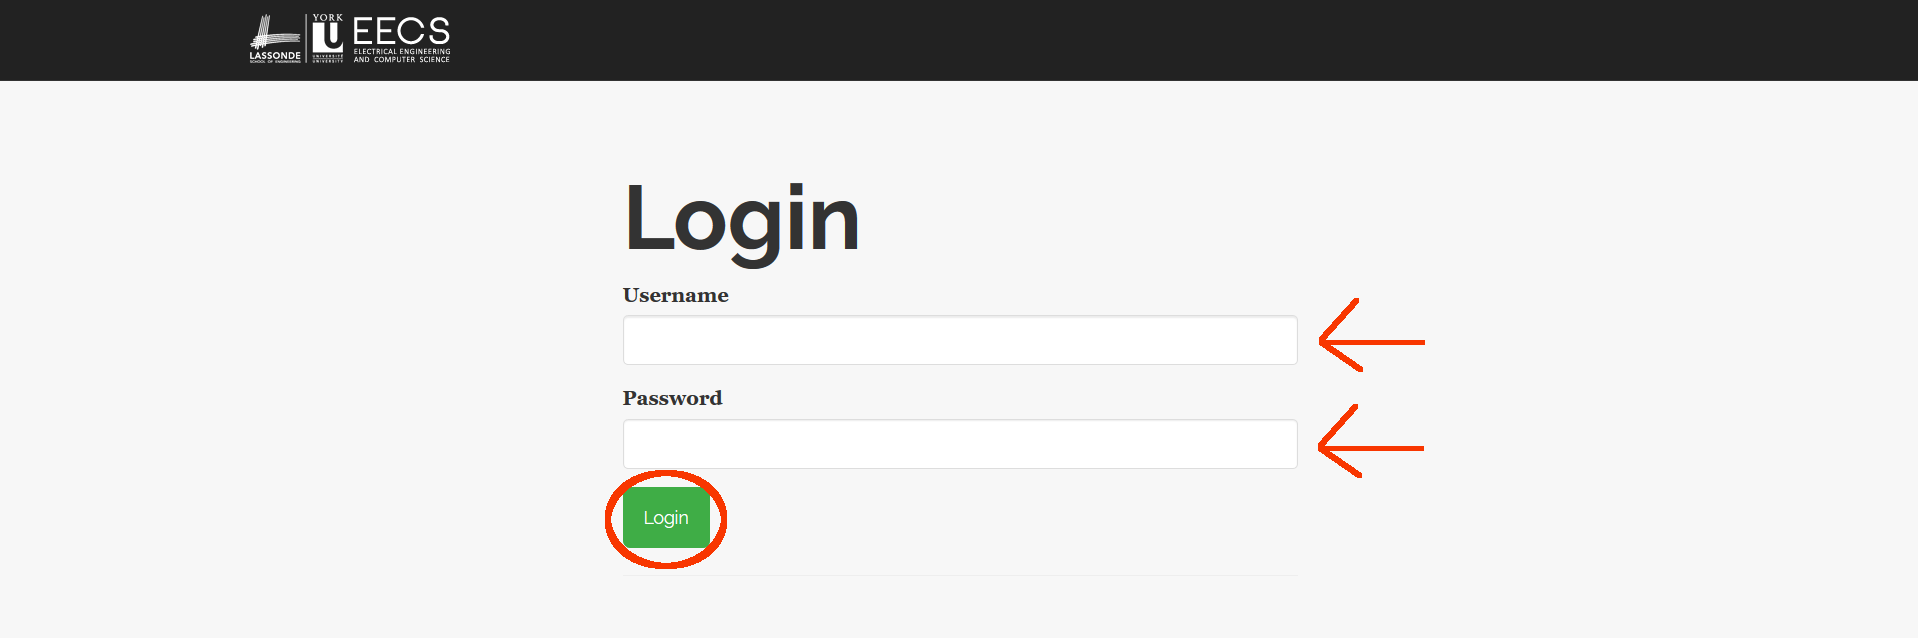
\includegraphics[width=.99\textwidth]{images/login.png}
\end{center}
\caption{Login Page}
\label{fig:login}
\end{figure}

\bigskip
\noindent \textbf{Note:} If the credentials you have provided are invalid you will be greeted with an error message.

\subsection{Selecting a Role}
The subsections below describe the methods for selecting the a role.

\subsubsection{Role Selection Page}
From the role selection page click on the ``Continue as Committee Member" button to be redirected to the committee member portal.

\begin{figure}[!htb]
\begin{center}
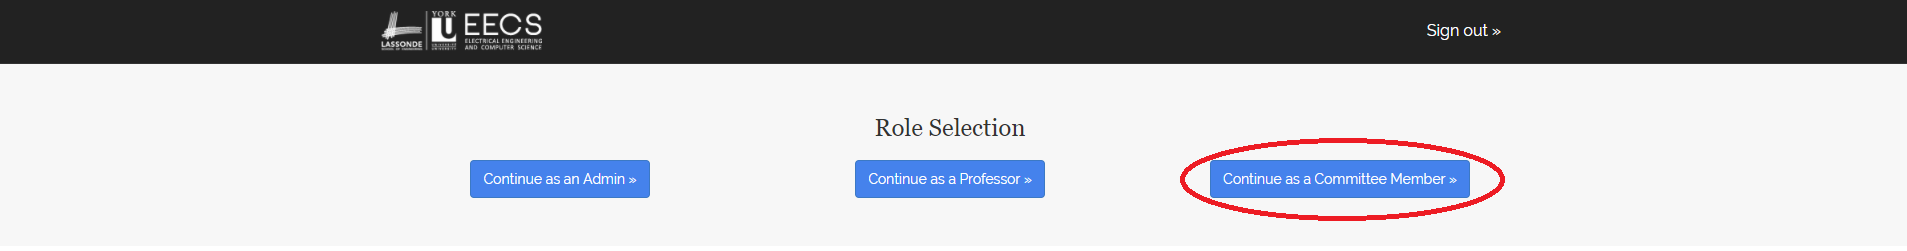
\includegraphics[width=.99\textwidth]{images/auth.png}
\end{center}
\caption{Role Selection Page}
\label{fig:role_selection1}
\end{figure}

\noindent \textbf{Note:} To access the administrator/committee/professor portal you must be granted access from an administrator.

\subsubsection{Navigation Bar}
If you have selected another role and wish to switch roles you will be presented with an option on the navigation bar. Click on the dropdown menu that displays your current role and click on your desired role.
\begin{figure}[!htb]
\begin{center}

\includegraphics[width=.99\textwidth]{images/role-selection2.png}
\end{center}
\caption{Switch Roles}
\label{fig:role_selection2}
\end{figure}

\noindent \textbf{Note:} To access the administrator/committee/professor portal you must be granted access from an administrator.

\subsection{User Settings}
\label{user-settings}
To customize personal user settings, simply click on the ``Settings" button from the navigation bar on any page. The following are the required fields when update personal user settings:
\begin{itemize}
\item Username
\item Last Name
\item First Name
\item Email
\end{itemize}

\begin{figure}[!htb]
\begin{center}
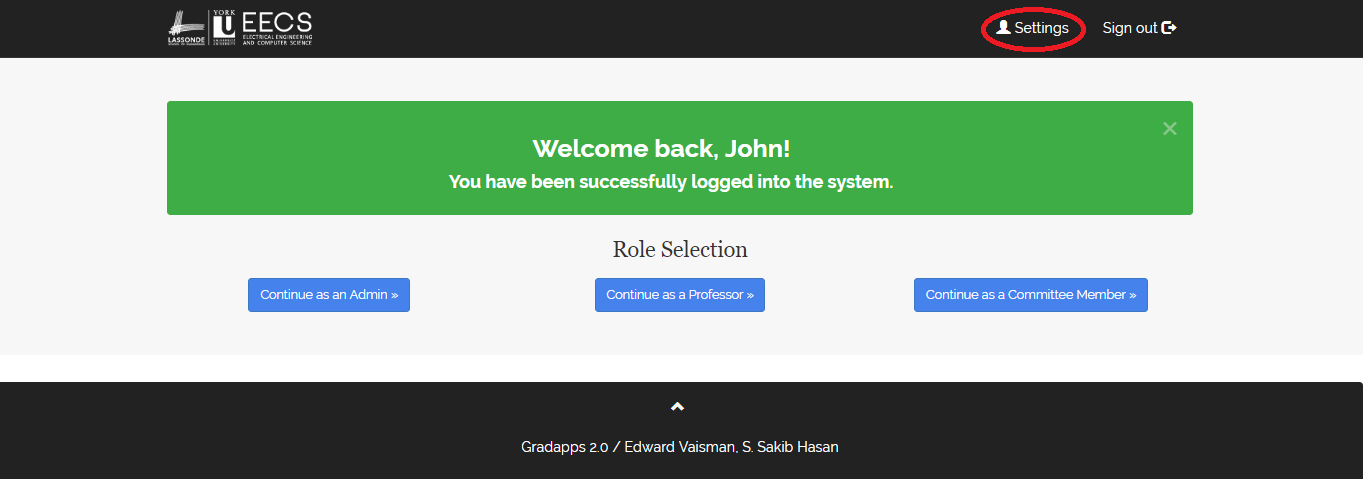
\includegraphics[width=.99\textwidth]{images/click_settings.png}
\end{center}
\caption{Open User Settings}
\label{fig:click_settings}
\end{figure}

\begin{figure}[!htb]
\begin{center}
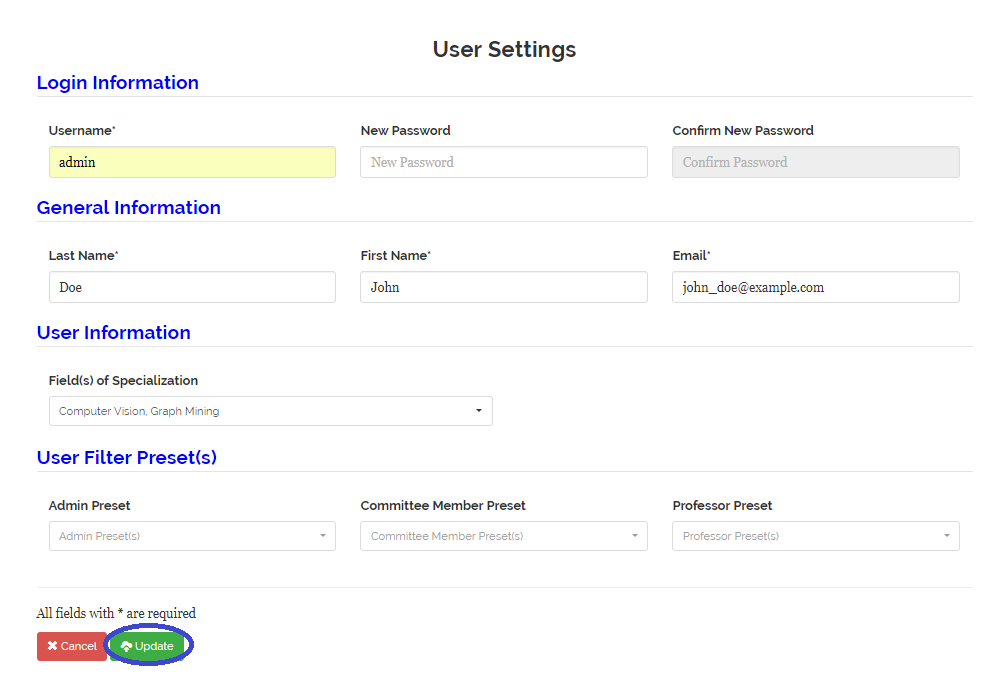
\includegraphics[width=.99\textwidth]{images/settings_form.png}
\end{center}
\caption{User Settings Form}
\label{fig:settings_form}
\end{figure}

\clearpage
\subsection{Logging Out}
To logout of the system, simply click on the ``Sign out" button from the navigation bar on any page.

\bigskip
\noindent \textbf{Note:} Idleness in the system for a maximum of 15 minute will cause the user session to be automatically terminated and the user will be logged out.

\begin{figure}[!htb]
\begin{center}
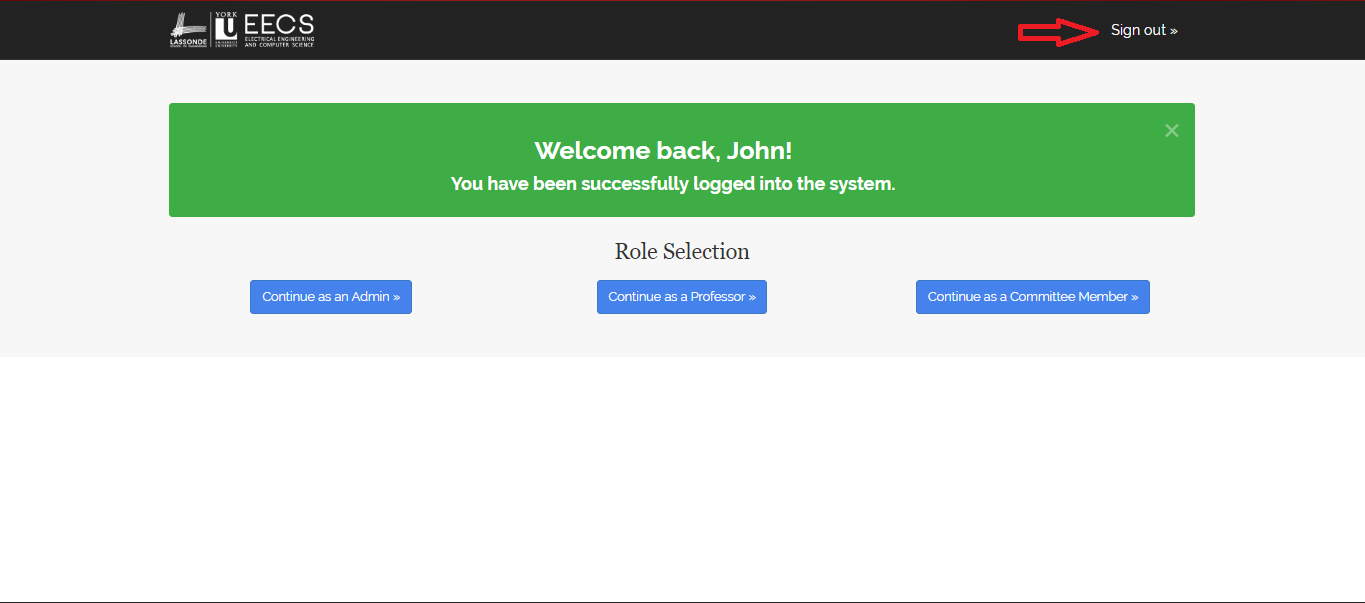
\includegraphics[width=.99\textwidth]{images/logout.png}
\end{center}
\caption{Logout of the System}
\label{fig:logout}
\end{figure}

%%%%%%%%%%%% ADMIN MANUAL %%%%%%%%%%%
\clearpage
\newpage
\section{Administrator}
This section provides a detailed description of the administrator system functions.

\subsection{Administrator Dashboard}

After logging in and selecting the \emph{Admin} role you will have access to the administrator dashboard. From the dashboard you can perform the following:
\begin{itemize}
\item Manage Users (Refer to section: \ref{m_user})
\begin{itemize}
\item Adding a new user
\item Remove an existing user
\item Assign a new role to an user
\item Removing a role from an user
\item Updating user information such as:
\begin{itemize}
\item Username
\item Password
\item Last Name
\item First Name
\item Email Address
\item Field(s) of Specialization
\end{itemize}
\item Deleting unwanted filter presets
\end{itemize}
\item Manage Applications (Refer to section: \ref{m_appls})
\begin{itemize}
\item Creating a new application
\item Deleting an existing application
\item Apply filtering on existing application(s)
\item Save presets on most used filter(s)
\item Export all or a set of application(s) to CSV
\item View application PDF file
\end{itemize}
\item Manage Reviews (Refer to section: \ref{m_reviews})
\begin{itemize}
\item Assign at most one reviewer for visa applicants
\item Assign at most two reviewer(s) for domestic applicants
\item Unassign reviews from an application
\item Dismiss submitted review from an application
\item View application PDF file
\end{itemize}
\end{itemize} 

\smallskip
\noindent More on each of the three management portals in the following sections.

\begin{figure}[!htb]
\begin{center}
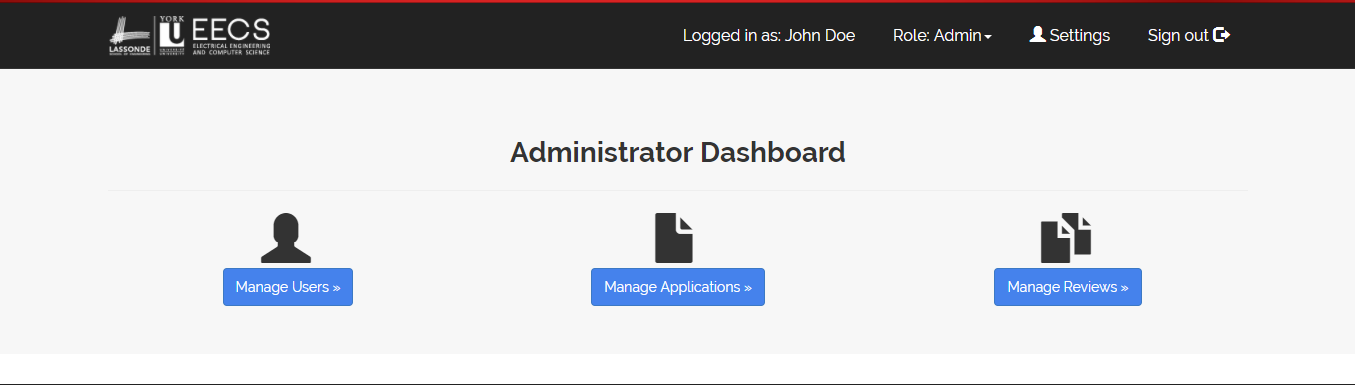
\includegraphics[width=.99\textwidth]{images/adm/admin_dash.png}
\end{center}
\caption{Administrator Dashboard}
\label{fig:adm/admin_dash}
\end{figure}

\smallskip
\noindent \textbf{Note:} Each of the management portal has a \emph{Go back to dashboard} link which upon clicking will bring back to the default dashboard.


%%%%%%%%% MANAGE USER %%%%%%%%%%
\newpage
\clearpage
\subsection{Manage Users} \label{m_user}
This section describes how you would add/remove a user, assign/unassign roles from a user and update user related information. To begin, from the administrator dashboard, click on \emph{Manage Users}.

\begin{figure}[!htb]
\begin{center}
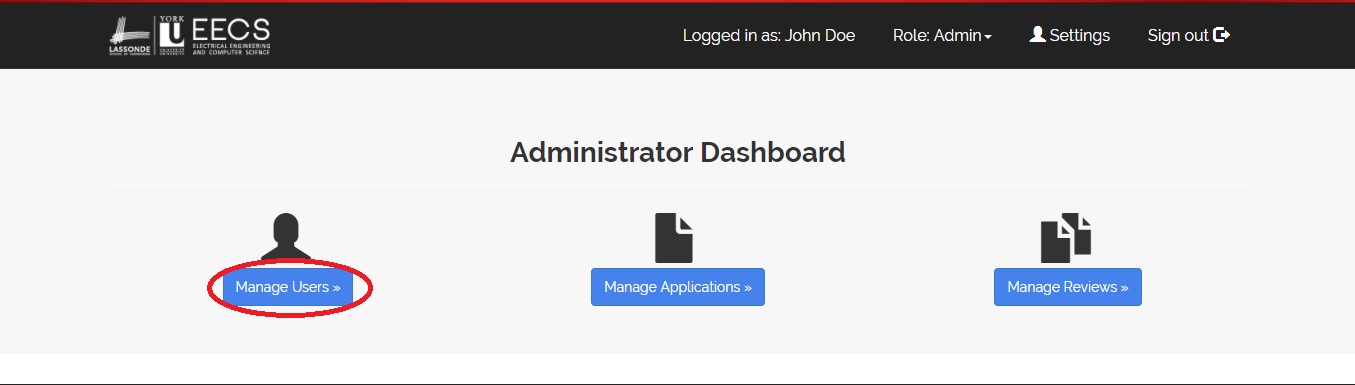
\includegraphics[width=.99\textwidth]{images/adm/mu/manage_user.png}
\end{center}
\caption{Click to Manage Users}
\label{fig:adm/manage_user}
\end{figure}

\subsubsection{Adding a user}
Once in the managing user portal, you can add a new user to the system. Adding a new user to the system requires you to give them a username (EECS username), generate a random password or make a password for the user, fill in basic user information (such as Last Name, First Name, Email Address, Field(s) of Specialization) and assign them a role. The following fields are required when creating a new user:
\begin{itemize}
\item Username
\item Password
\item Last Name
\item First Name
\item Email
\item Role(s)
\end{itemize}

\smallskip
\noindent \textbf{Note:} Username for a user is unique and hence trying to create a user with an existing username will not allow the new user to be created.

\begin{figure}[!htb]
\begin{center}
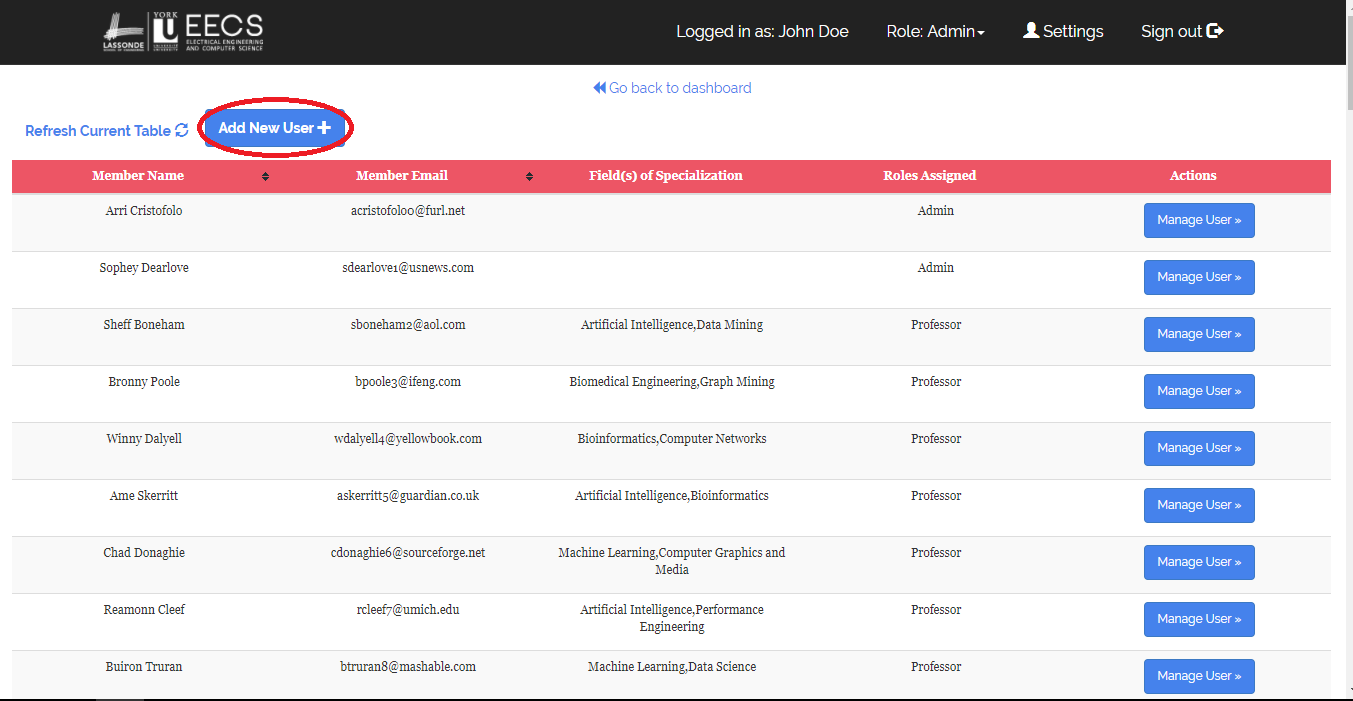
\includegraphics[width=.99\textwidth]{images/adm/mu/new_user_click.png}
\end{center}
\caption{Click to create a user}
\label{fig:adm/new_user_click}
\end{figure}

\begin{figure}[!htb]
\begin{center}
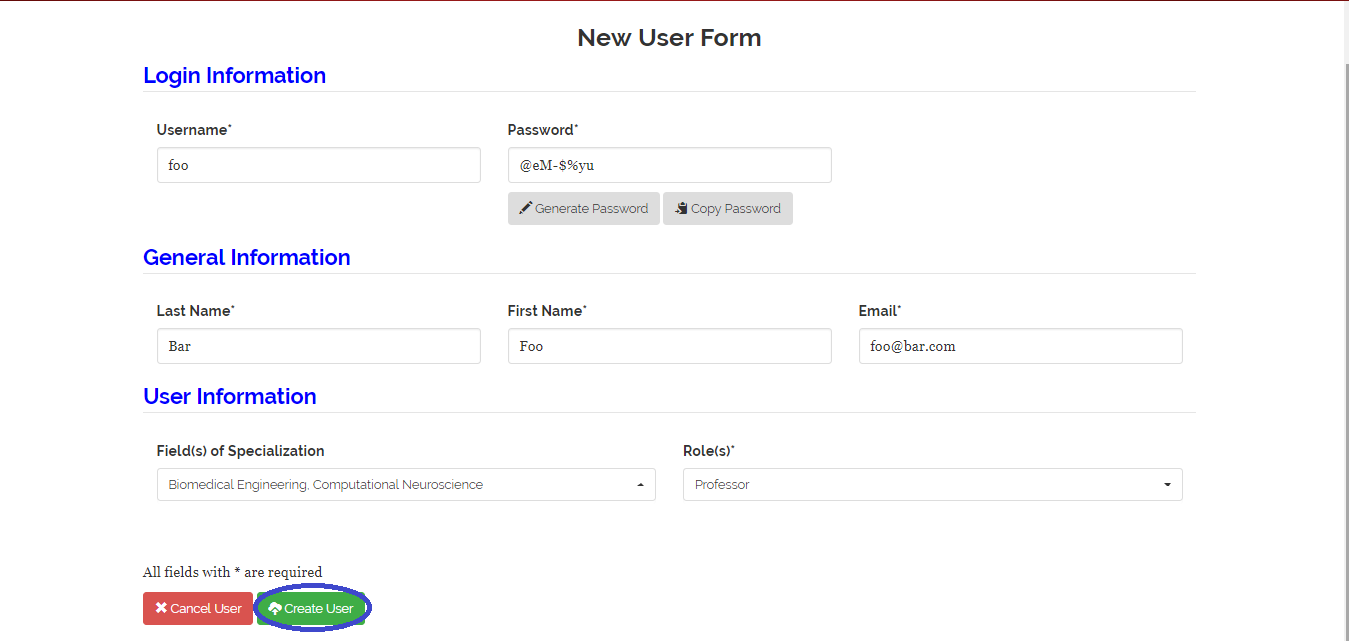
\includegraphics[width=.99\textwidth]{images/adm/mu/fill_in_user.png}
\end{center}
\caption{Filling in user information}
\label{fig:adm/fill_in_user}
\end{figure}

\clearpage
\subsubsection{Edit existing user}
Once in the managing user portal, you can edit an existing user. Editing includes updating user information, assigning/unassigning roles or removing the user completely from the system.

\begin{figure}[!htb]
\begin{center}
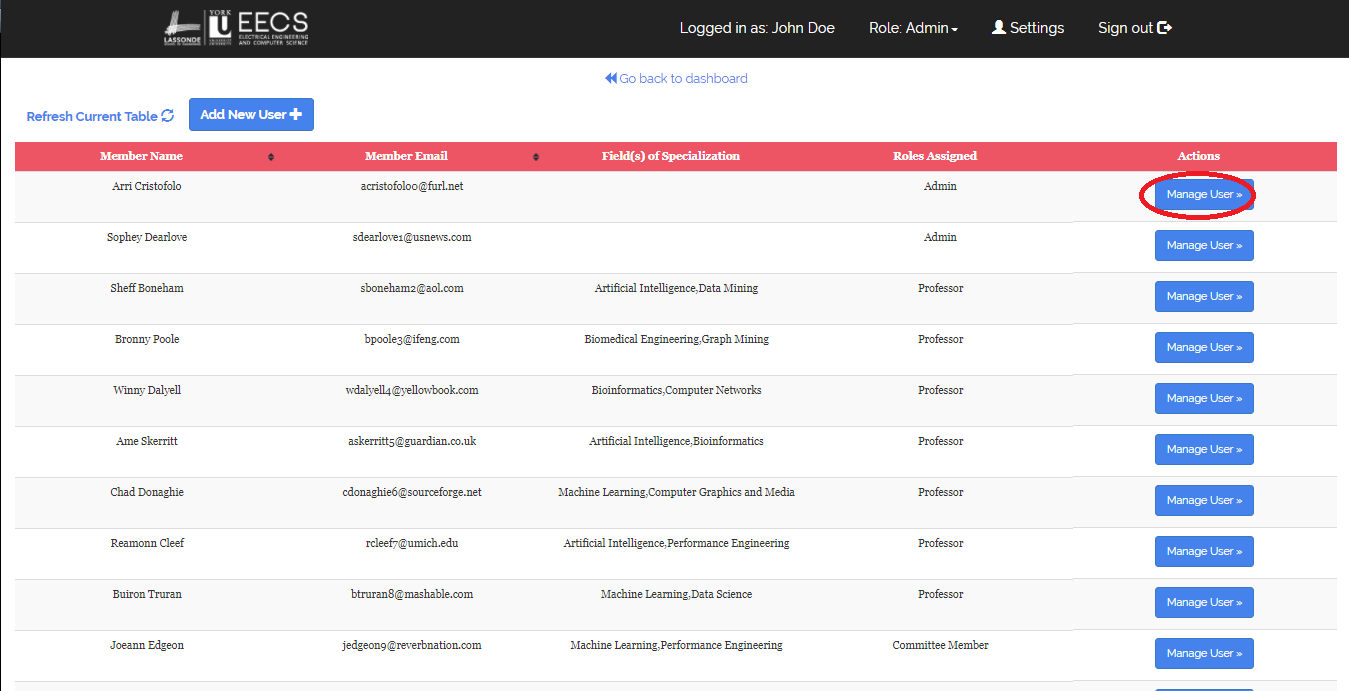
\includegraphics[width=.99\textwidth]{images/adm/mu/edit_user.png}
\end{center}
\caption{Click to edit an user}
\label{fig:adm/edit_user}
\end{figure}

\smallskip
\noindent \textbf{Note:} An administrator cannot edit their own user settings from the manage user portal. Another administrator has to edit it for them. However, they can update their own personal settings like any other user from the \emph{Settings} menu in the navbar. 

\begin{figure}[!htb]
\begin{center}
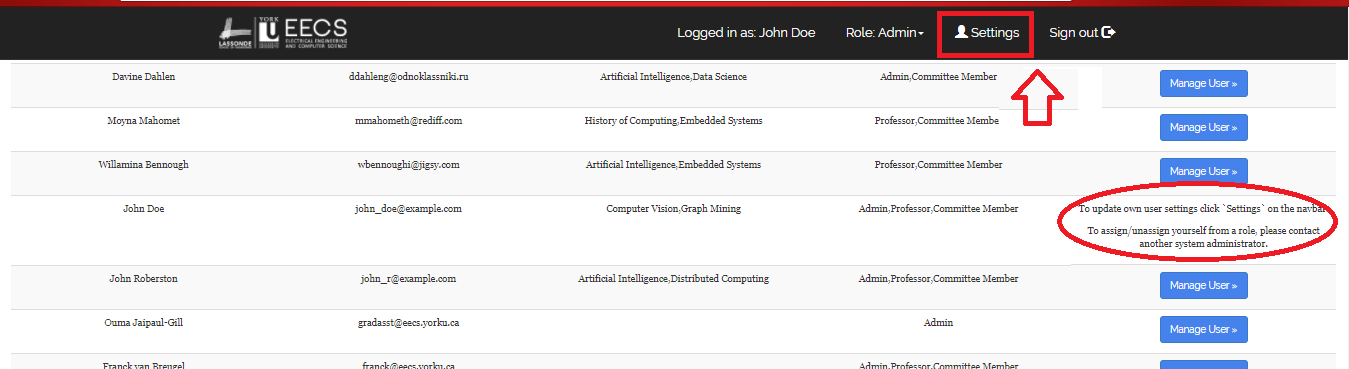
\includegraphics[width=.99\textwidth]{images/adm/mu/edit_own_user.png}
\end{center}
\caption{Editing own user settings}
\label{fig:adm/edit_own_user}
\end{figure}

\clearpage
\subsubsection{Remove a user}
To remove an existing user from the system, click on the \emph{Manage User} button as shown above for the corresponding user. Then click on the trash can button at the bottom of the page as shown.

\smallskip
\noindent \textbf{Note:} As an administrator you can only remove other users. You cannot remove yourself from the system. Another administrator has to remove you in that case.

\begin{figure}[!htb]
\begin{center}
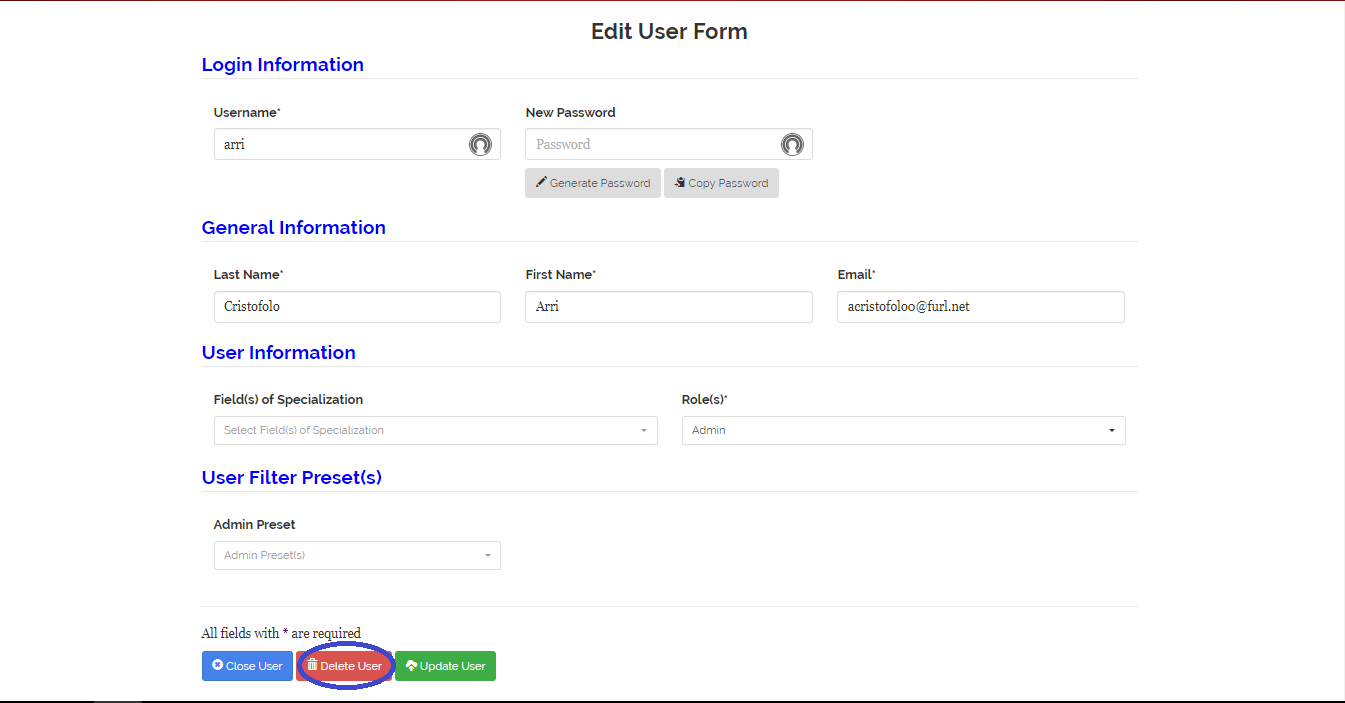
\includegraphics[width=.99\textwidth]{images/adm/mu/remove_user.png}
\end{center}
\caption{Removing an user}
\label{fig:adm/remove_user}
\end{figure}

\clearpage
\subsubsection{Assign/Unassign roles}
To assign or unassign a role from an existing user from the system, click on the \emph{Manage User} button as shown above for the corresponding user. Then select or de-select the role you want to assign or unassign for the user.

\smallskip
\noindent \textbf{Note:} A user must have at least one role assigned to them at all times.

\begin{figure}[!htb]
\begin{center}
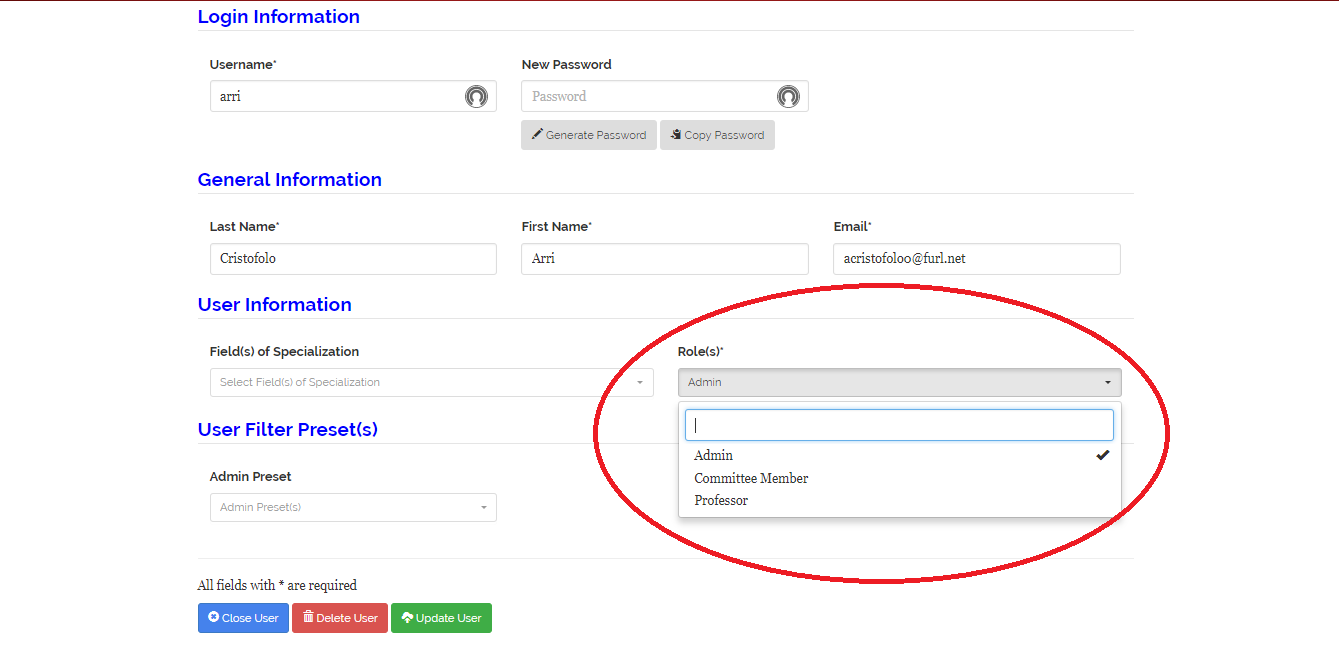
\includegraphics[width=.99\textwidth]{images/adm/mu/edit_roles.png}
\end{center}
\caption{Assign/Unassign roles}
\label{fig:adm/edit_roles}
\end{figure}

\clearpage
\subsubsection{Update User Information}
As an administrator you can update user information. To update user information for an existing user, click on the \emph{Manage user} button as shown above for the corresponding user. Then click on the upload button at the bottom of the page as shown. The following fields are required when updating a user information:
\begin{itemize}
\item Username
\item Last Name
\item First Name
\item Email
\item Role(s)
\end{itemize}

\smallskip
\noindent \textbf{Note:} All required fields are needed to be filled when editing an user.

\begin{figure}[!htb]
\begin{center}
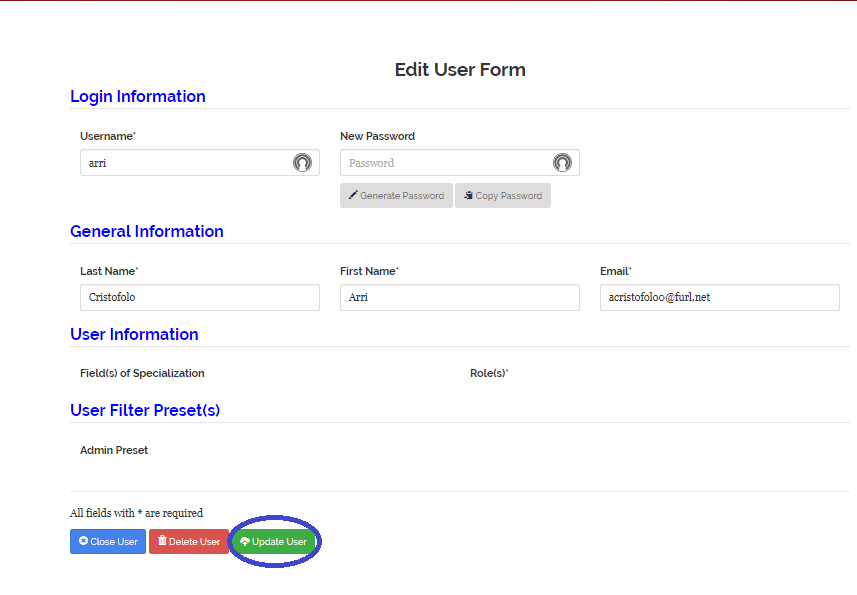
\includegraphics[width=.9\textwidth]{images/adm/mu/update_user.png}
\end{center}
\caption{Updating an user}
\label{fig:adm/update_user}
\end{figure}

\clearpage
\subsubsection{Remove Unwanted Filter Presets}
As an administrator you can remove unwanted filter presets for a particular user. To remove such presets for an existing user, click on the \emph{Manage user} button as shown above for the corresponding user. Then simply unchecking the preset from the dropdown will permanently remove the preset for the user.

\begin{figure}[!htb]
\begin{center}
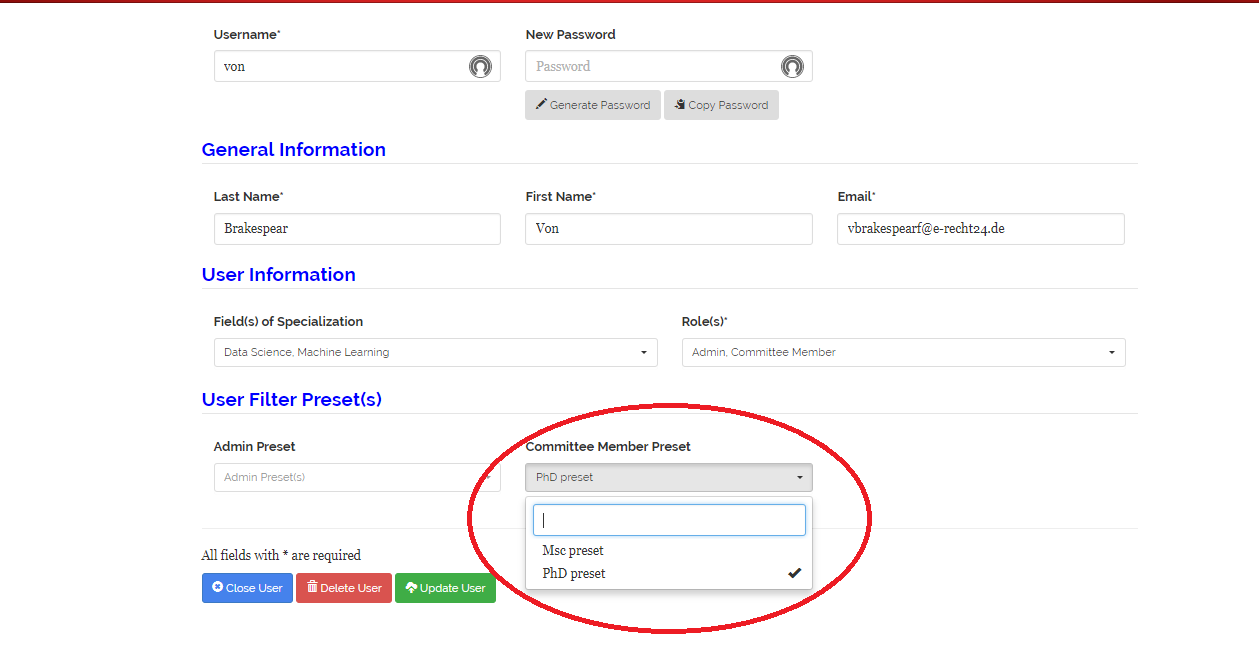
\includegraphics[width=.99\textwidth]{images/adm/mu/remove_preset.png}
\end{center}
\caption{Remove Filter Presets}
\label{fig:adm/remove_preset}
\end{figure}


\subsubsection{Sorting the Table}
If you wish to sort the table displayed simply click on the columns that display arrows next to the name. The table can be sorted in Ascending/Descending order described below.

\begin{itemize}
\item \textbf{Member Name:} Descending Order = Z to A, Ascending order = A to Z
\item \textbf{Member Email:} Descending Order = Z to A, Ascending order = A to Z
\end{itemize}

\textbf{Pro-tip:} To sort by multiple columns hold the shift key while clicking on the columns.

%%%%%%%%%%%% MANAGE APPLICATIONS %%%%%%%%%%%%

\newpage
\clearpage
\subsection{Manage Applications} \label{m_appls}
This section describes how you would create/delete an application, export applications to CSV, apply filtering on application(s), save most used filter(s) as preset and viewing application PDF file. To begin, from the administrator dashboard, click on \emph{Manage Applications}.

\begin{figure}[!htb]
\begin{center}
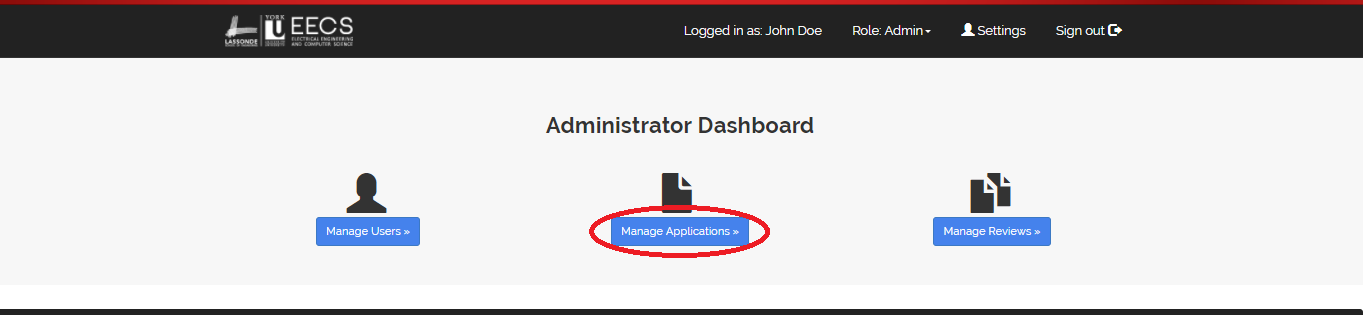
\includegraphics[width=.99\textwidth]{images/adm/ma/manage_app.png}
\end{center}
\caption{Click to Manage Applications}
\label{fig:adm/manage_app}
\end{figure}

\subsubsection{Create an application} \label{c_appl}
Once in the managing application portal, you can create a new application and upload all necessary documents. Creating a new application requires you to upload the application file, filling out general application information, previous grades, application information and finally assigning a one or more reviewer from the admission graduate committee. The following fields are required when creating a new application:
\begin{itemize}
\item Application File
\item Session
\item Student Number
\item Last Name
\item First Name
\item Email
\item Gender
\item GPA
\item Visa Status
\item Degree Applied For
\item Field(s) of Interest
\item Preferred Professor(s)
\end{itemize}

\begin{figure}[!htb]
\begin{center}
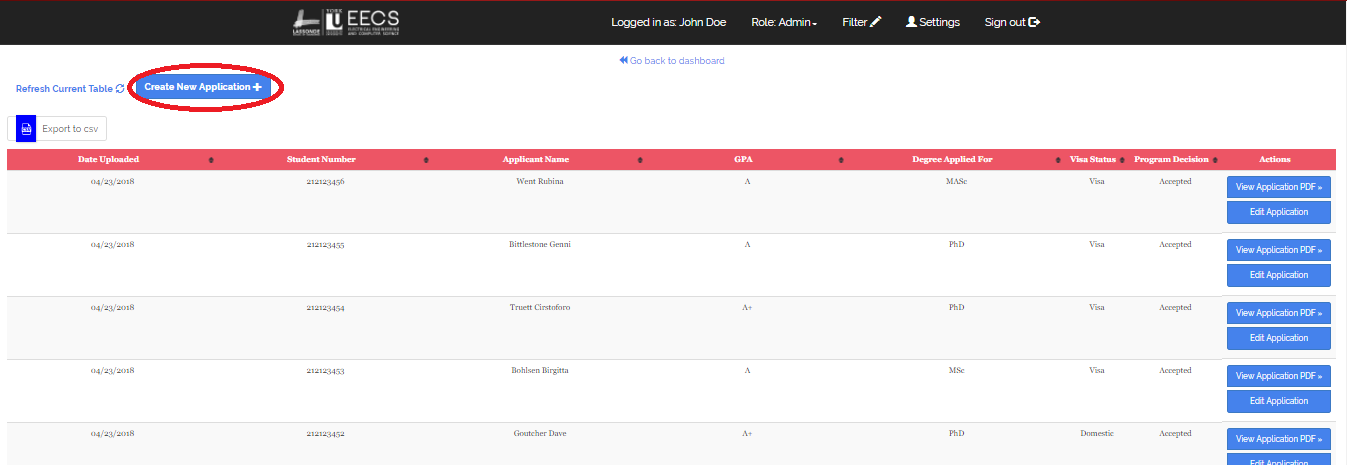
\includegraphics[width=.99\textwidth]{images/adm/ma/new_app_click.png}
\end{center}
\caption{Click to create a application}
\label{fig:adm/new_app_click}
\end{figure}

\clearpage
\begin{figure}[!htb]
\begin{center}
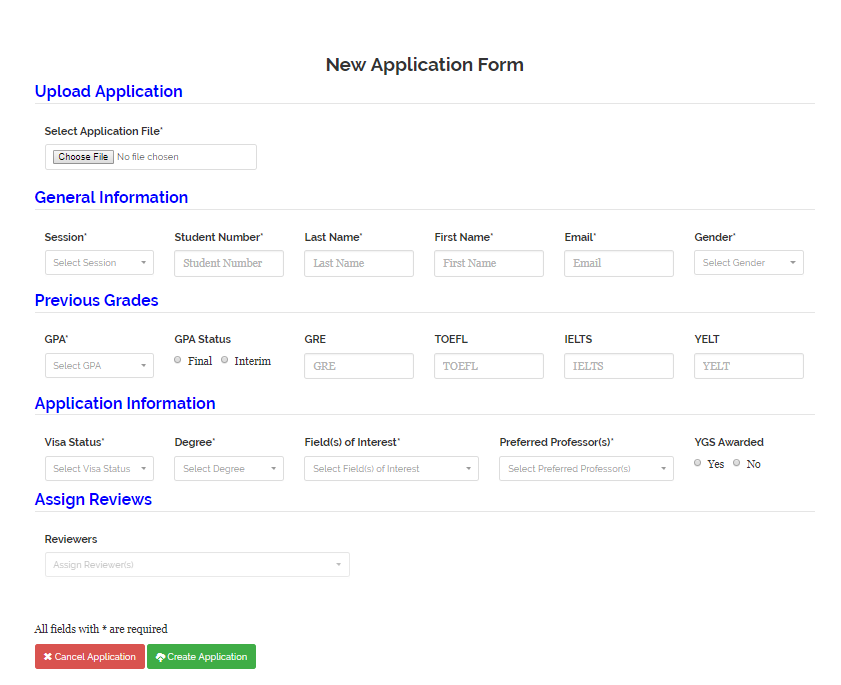
\includegraphics[width=.99\textwidth]{images/adm/ma/fill_in_app.png}
\end{center}
\caption{Filling in application}
\label{fig:adm/fill_in_app}
\end{figure}

\smallskip
\noindent \textbf{Note:} The maximum application file size for upload is set to 4MB and only accepted format of file accepted is PDF.

\clearpage
\subsubsection{Edit existing application}
Once in the managing application portal, you can edit an existing application. Editing includes updating all attributes specified in the previous section (refer to Section \ref{c_appl}) plus additional attributes such as professor(s) that have contacted or requested the student, the program decision, the student decision and etc.

\begin{figure}[!htb]
\begin{center}
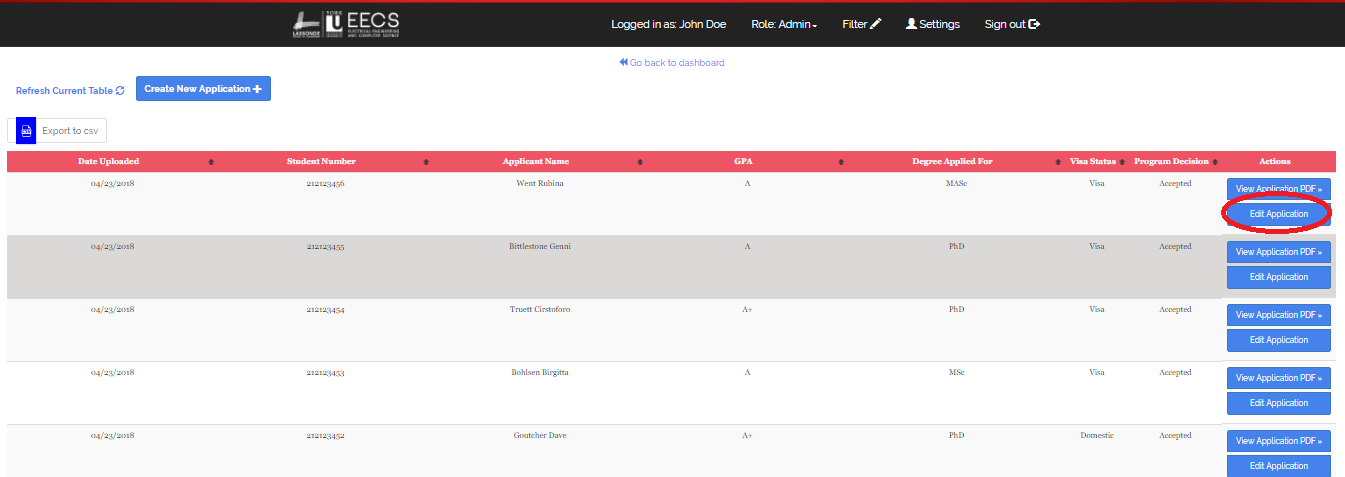
\includegraphics[width=.99\textwidth]{images/adm/ma/edit_appl.png}
\end{center}
\caption{Click to edit an application}
\label{fig:adm/edit_appl}
\end{figure}

\clearpage
\subsubsection{Remove an application}
To remove an existing application from the system, click on the \emph{Manage Applications} button as shown above for the corresponding application. Then click on the trash can button at the bottom of the page as shown.

\begin{figure}[!htb]
\begin{center}
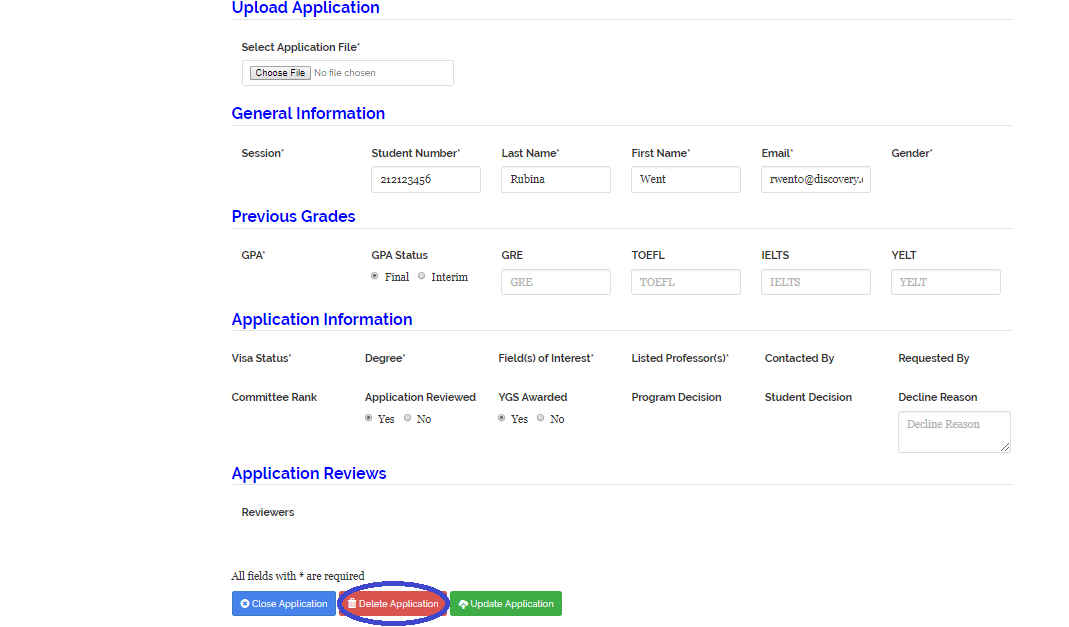
\includegraphics[width=.99\textwidth]{images/adm/ma/remove_appl.png}
\end{center}
\caption{Removing an application}
\label{fig:adm/remove_appl}
\end{figure}

\clearpage
\subsubsection{Update an application}
To update an existing application from the system, click on the \emph{Manage Applications} button as shown above for the corresponding application. Then click on the upload button at the bottom of the page as shown. The fields that are required when editing an application is the same as when creating an application.

\begin{figure}[!htb]
\begin{center}
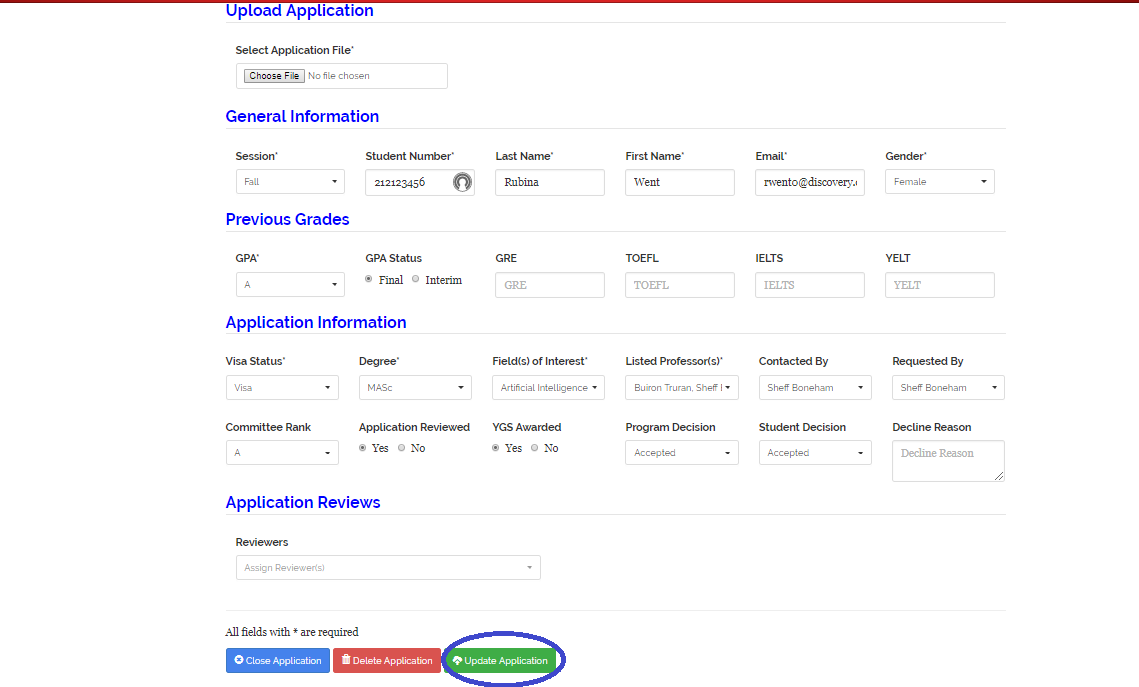
\includegraphics[width=.99\textwidth]{images/adm/ma/update_appl.png}
\end{center}
\caption{Updating an application}
\label{fig:adm/update_appl}
\end{figure}

\clearpage
\subsubsection{Export Application(s)}
Once in the managing application portal, you can export all or a set of application(s) in CSV format. To achieve a set of applications simply use filtering to narrow down the application result. Clicking on the \emph{Export to CSV} button will download all selected application into a CSV file.

\begin{figure}[!htb]
\begin{center}
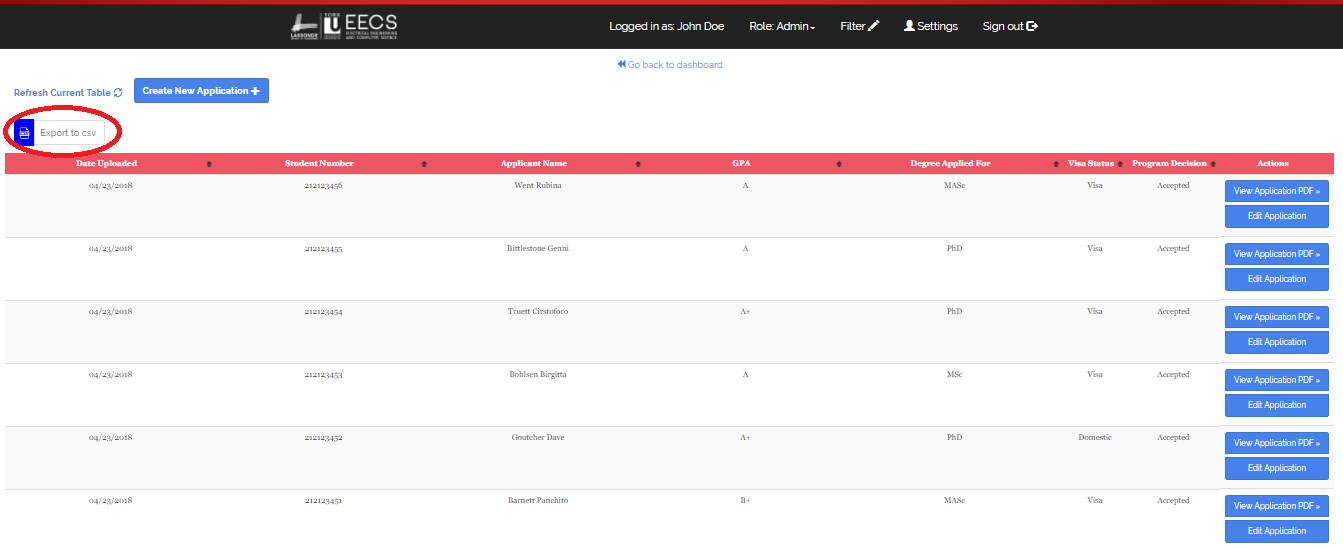
\includegraphics[width=.99\textwidth]{images/adm/ma/export_appl.png}
\end{center}
\caption{Exporting application(s)}
\label{fig:adm/export_appl}
\end{figure}

\clearpage
\subsubsection{View Application PDF}
Once in the managing application portal, you can chose to view the PDF formatted file of the application. Clicking on the \emph{View Application PDF} for the corresponding application will open a new tab along with the pdf file.

\begin{figure}[!htb]
\begin{center}
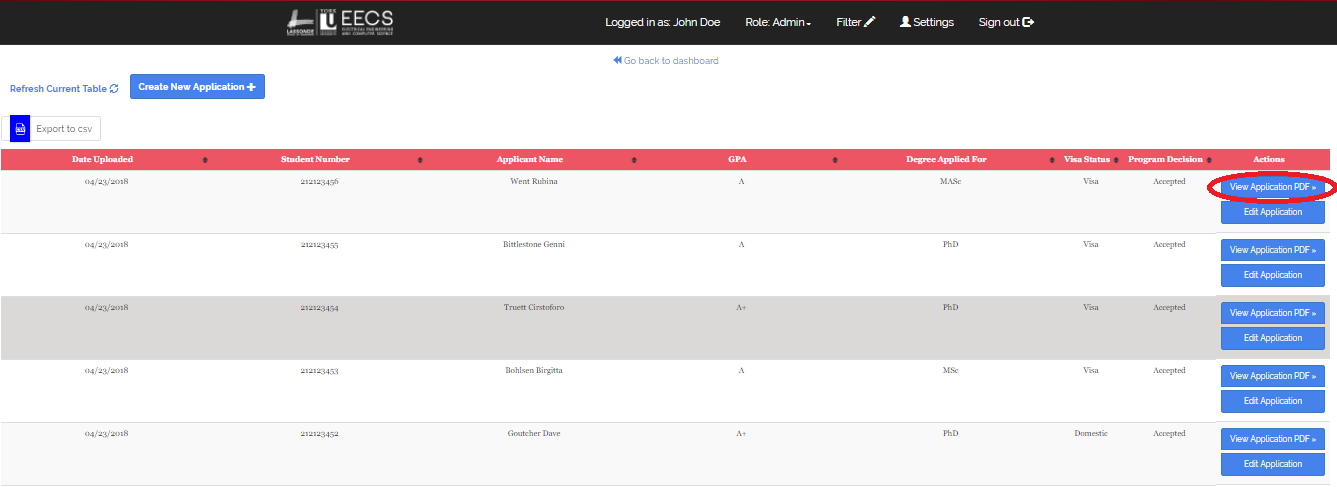
\includegraphics[width=.9\textwidth]{images/adm/ma/view_appl_app.png}
\end{center}
\caption{Viewing Application PDF}
\label{fig:adm/view_appl_app}
\end{figure}

\begin{figure}[!htb]
\begin{center}
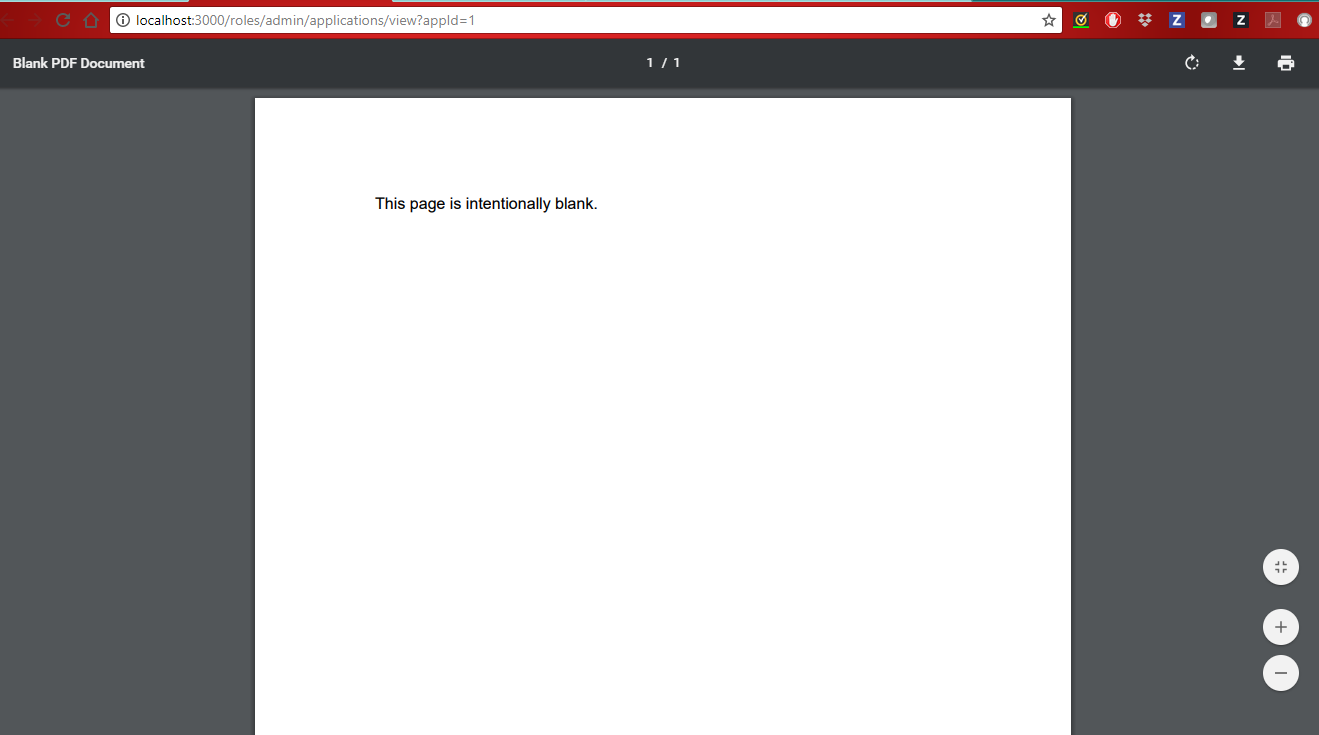
\includegraphics[width=.9\textwidth]{images/adm/ma/appl_pdf.png}
\end{center}
\caption{Application PDF}
\label{fig:adm/appl_pdf}
\end{figure}

\clearpage
\subsubsection{Filtering the Table}
This section describes how you would use/build/save/load a filter on the review table.

\begin{enumerate}


\item \textbf{Opening the Modal} To begin with filtering you must open the modal. To do so click on the ``Filter" button on the navigation bar.

\begin{figure}[!htb]
\begin{center}
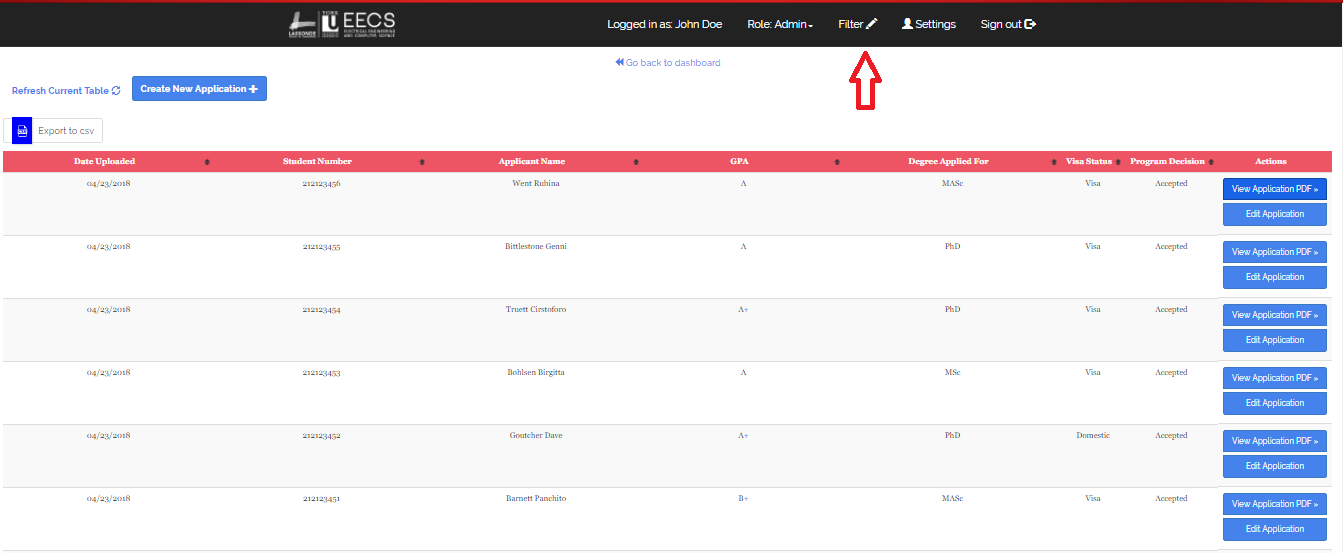
\includegraphics[width=.99\textwidth]{images/adm/ma/open_modal.png}
\end{center}
\caption{Opening the  Modal}
\label{fig:adm/open_modal}
\end{figure}

\clearpage

\begin{figure}[!htb]
\begin{center}
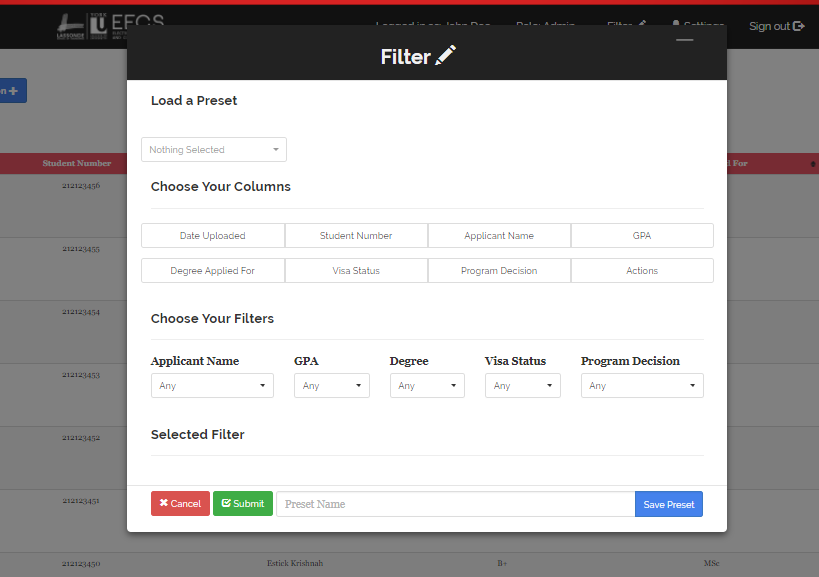
\includegraphics[width=.99\textwidth]{images/adm/ma/default_filter_view.png}
\end{center}
\caption{Filter View}
\label{fig:adm/filter_view}
\end{figure}

\item \textbf{Choose Your Columns} Once the modal is opened you can then choose the columns you wish to be displayed on the table. To do so, click on the button indicating which column you wish to see. Once clicked the button will display the order that column will appear in the table.

\begin{figure}[!htb]
\begin{center}
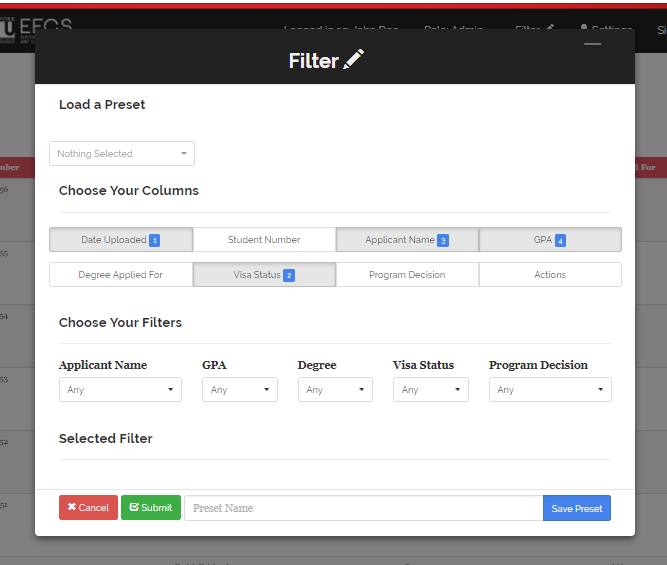
\includegraphics[width=.99\textwidth]{images/adm/ma/selected_col.png}
\end{center}
\caption{Choose Your Columns}
\label{fig:adm/choose_columns}
\end{figure}

\smallskip
\noindent \textbf{Note:} Not selecting any column will use the same columns and order as the default table. If the \emph{Actions} column is not selected it will automatically be placed as the right most column.

\clearpage
\item \textbf{Choose Your Filters} After selecting your columns, you can then choose the attributes by which you wish to filter your table. Begin by clicking on the drop down of the attribute you wish to filter and select an option from a list of generated options.

\begin{figure}[!htb]
\begin{center}
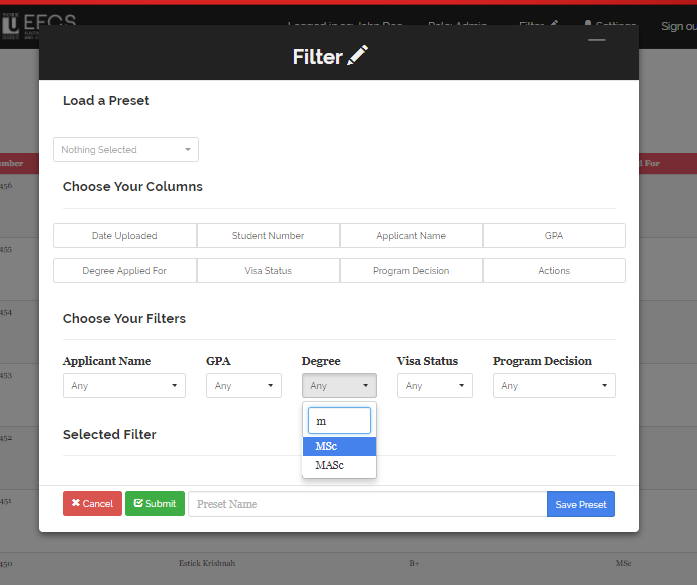
\includegraphics[width=.99\textwidth]{images/adm/ma/selected_filter.png}
\end{center}
\caption{Choose Your Filters}
\label{fig:adm/choose_filters}
\end{figure} 

\smallskip
\noindent \textbf{Note:} You can use the search bar to help locate values. Begin by typing in the text box displayed. You can only select an option that appears in the dropdown.

\clearpage
\item \textbf{Submitting a Filter} Once you have chosen your columns and filter attributes confirm your filter by reading the text under ``Selected Filter'' and click ``Submit". The text under the ``Selected Filter'' will change based on your filter attributes.

\begin{figure}[!htb]
\begin{center}
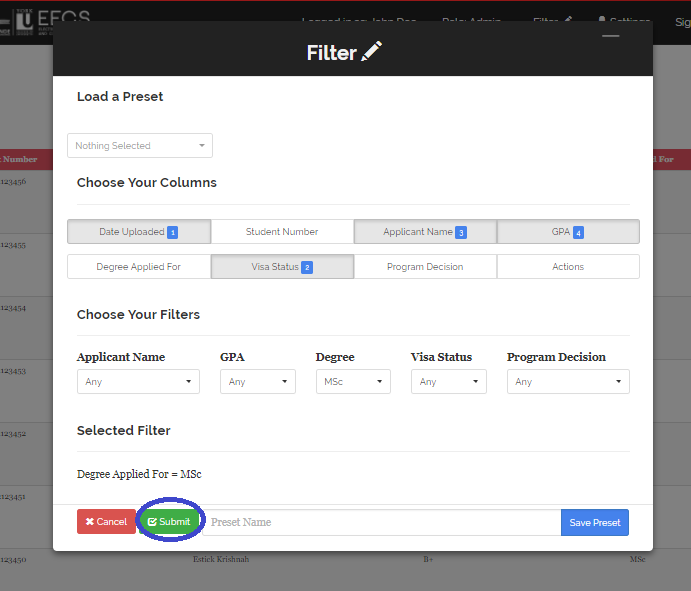
\includegraphics[width=.99\textwidth]{images/adm/ma/submit_filter.png}
\end{center}
\caption{Submit Filter}
\textbf{Note}: When submitting a filter with no selected filters, the default table will be loaded.
\label{fig:adm/submit_filter}
\end{figure}

\begin{figure}[!htb]
\begin{center}
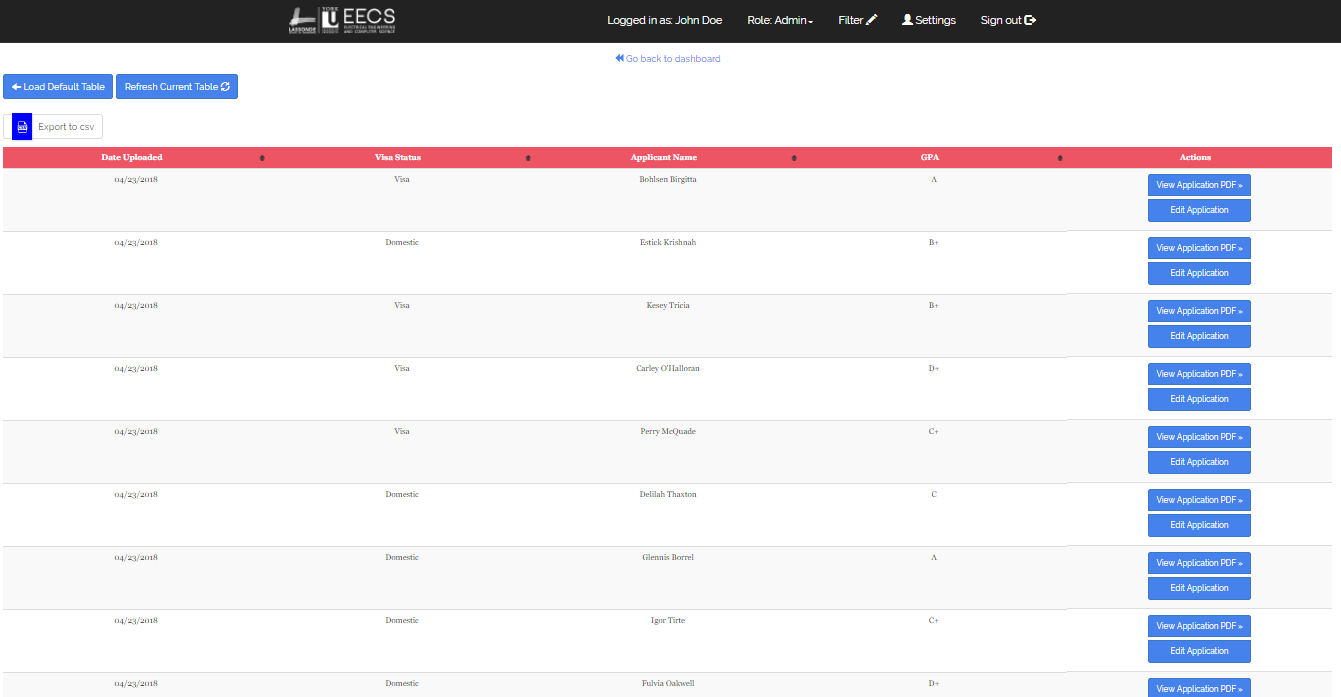
\includegraphics[width=.99\textwidth]{images/adm/ma/example_filter_table.png}
\end{center}
\caption{Resulted Table After Applying Filter}
\label{fig:adm/resulted_table}
\end{figure}

\clearpage
\item \textbf{Saving a Filter} Once you have chosen your columns and filter attributes confirm your filter by reading the text under ``Selected Filter'' and give the preset a name by typing in the text box between the ``Submit'' and the ``Save Preset'' button. Once that is done click ``Save Preset''.

\begin{figure}[!htb]
\begin{center}
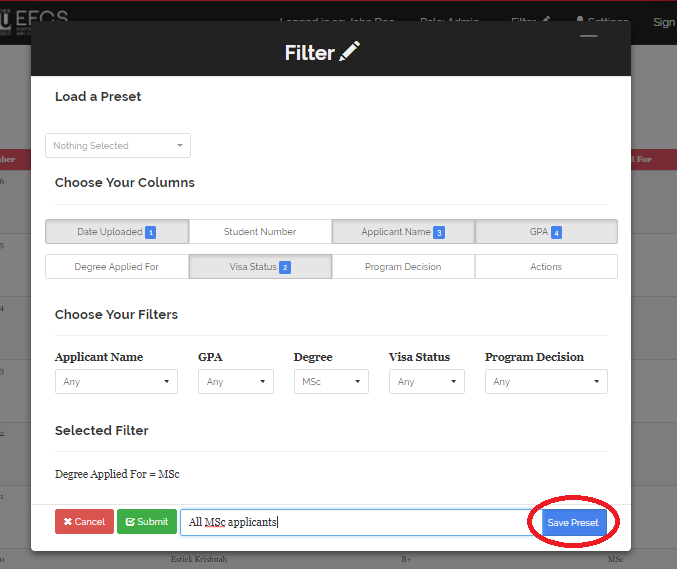
\includegraphics[width=.99\textwidth]{images/adm/ma/saving_preset.png}
\end{center}
\caption{Save a Filter}
\label{fig:adm/save_filter}
\end{figure}

\smallskip
\noindent Once you have saved a filter you will be provided with a new table to match your filter and it will appear in the dropdown to be used for loading a filter.

\smallskip
\noindent \textbf{Pro-tip:} You can update a filter by typing in the same name as an existing filter.

\clearpage
\item \textbf{Loading a Filter} To load a saved filter click the dropdown under ``Load a Preset'' and select the preset you wish to use. Once selected the modal will auto-populate.

\begin{figure}[!htb]
\begin{center}
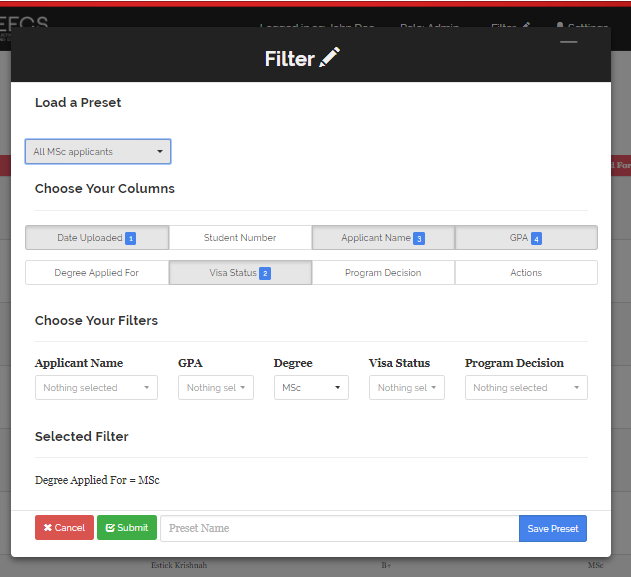
\includegraphics[width=.99\textwidth]{images/adm/ma/load_preset.png}
\end{center}
\caption{Loading a Filter}
\label{fig:adm/save_filter}
\end{figure}

\smallskip
\noindent \textbf{Pro-tip:} Create a preset called \emph{Default} with no columns or filters selected. You can then use this to load the default table or help clear any data you put in the modal.

\end{enumerate}

\clearpage
\subsubsection{Sorting the Table}
If you wish to sort the table displayed simply click on the columns that display arrows next to the name. The table can be sorted in Ascending/Descending order described below.
\begin{itemize}
\item \textbf{Date Uploaded:} Descending Order = Newest - Oldest, Ascending order = Oldest - Newest
\item \textbf{Student Number:} Descending Order = Largest to Smallest, Ascending order = Smallest to Largest
\item \textbf{Applicant Name:} Descending Order = Z to A, Ascending order = A to Z
\item \textbf{GPA:} Descending Order = A+ to F, Ascending order = F to A+
\item \textbf{Degree Applied For:} Descending Order = Z to A, Ascending order = A to Z
\item \textbf{Program Decision:} Descending Order = Z to A, Ascending order = A to Z
\end{itemize}
\textbf{Pro-tip:} To sort by multiple columns hold the shift key while clicking on the columns.

\bigskip
\noindent \textbf{Note}: Ordering fields can be done on both filtered and unfiltered application lists.

\bigskip
\noindent The following images depict how to order review applications using the \emph{Student Number} field in ascending and descending order.

\begin{figure}[!htb]
\begin{center}
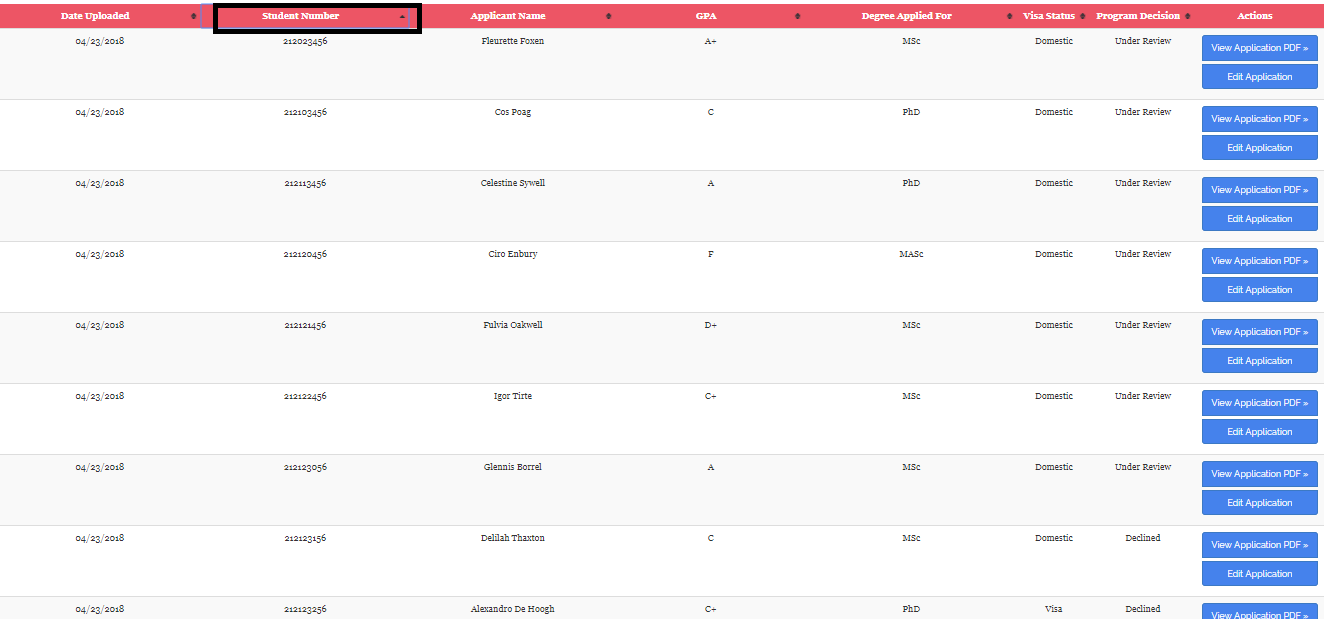
\includegraphics[width=.8\textwidth]{images/adm/ma/order_ascending.png}
\end{center}
\caption{Ascending order of Student Number field}
\label{fig:adm/order_ascending}
\end{figure}

\begin{figure}[!htb]
\begin{center}
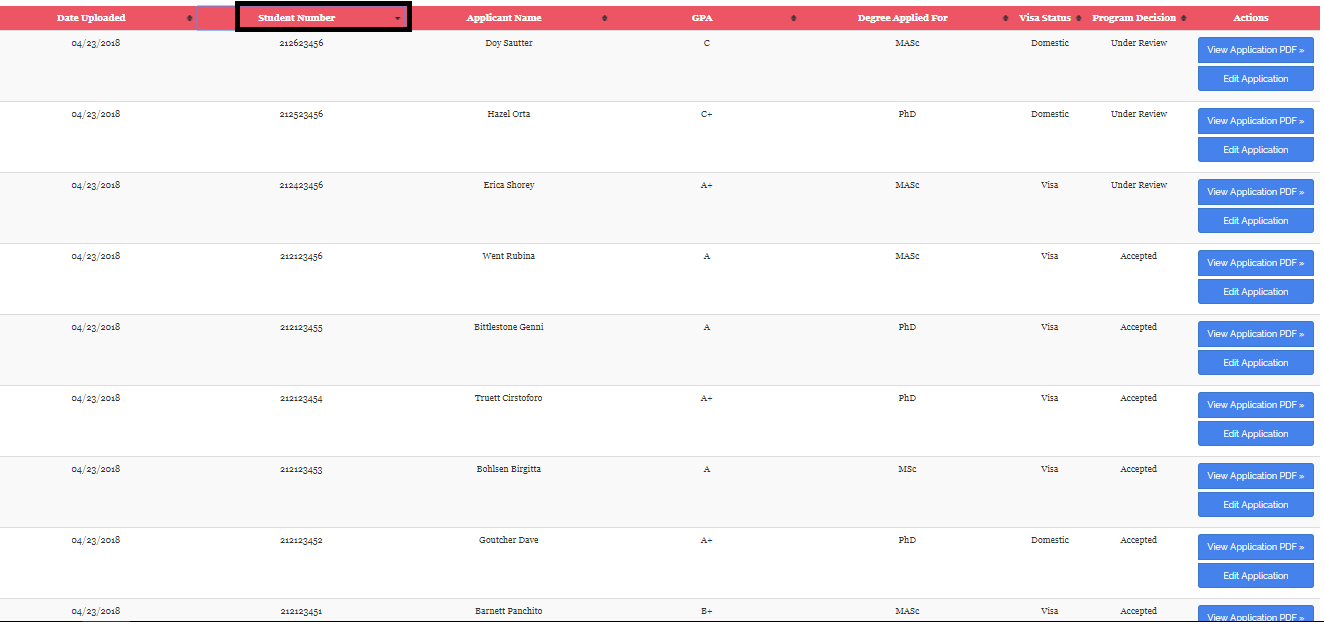
\includegraphics[width=.99\textwidth]{images/adm/ma/order_descending.png}
\end{center}
\caption{Descending order of Student Number field}
\label{fig:adm/order_descending}
\end{figure}

\begin{figure}[!htb]
\begin{center}
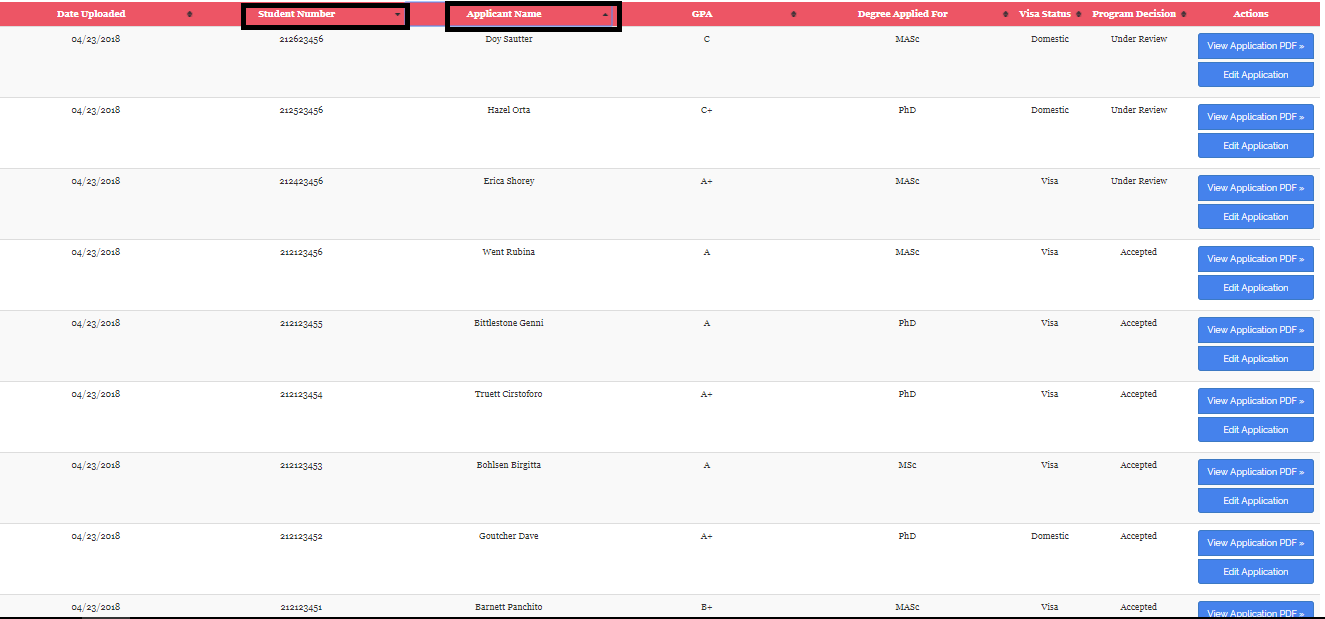
\includegraphics[width=.99\textwidth]{images/adm/ma/multiple_order.png}
\end{center}
\caption{Ordering using multiple fields}
\label{fig:adm/multiple_order}
\end{figure}

%%%%%%%%%%%% MANAGE REVIEWS %%%%%%%%%%%%

\newpage
\clearpage
\subsection{Manage Reviews} \label{m_reviews}
This section describes how you would assign, unassign or dismiss reviews for an application and apply filter on review applications. To begin, from the administrator dashboard, click on \emph{Manage Reviews}.

\begin{figure}[!htb]
\begin{center}
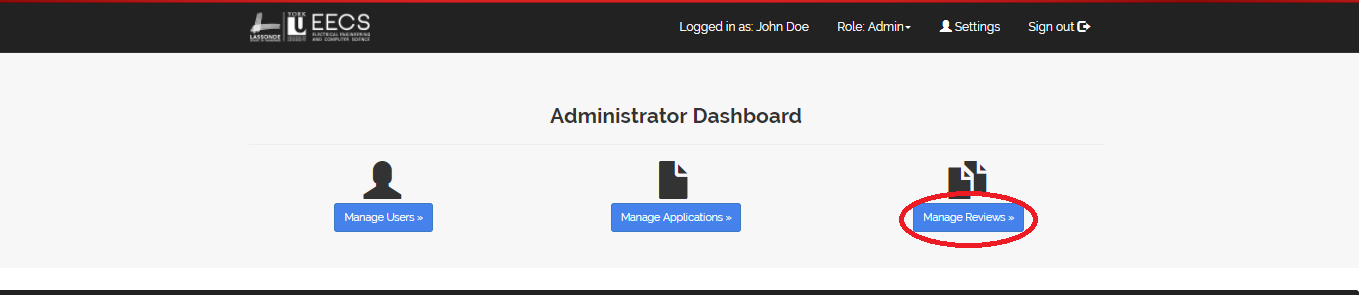
\includegraphics[width=.99\textwidth]{images/adm/mr/manage_review.png}
\end{center}
\caption{Click to Manage Reviews}
\label{fig:adm/manage_review}
\end{figure}


\subsubsection{Assign Review}
Once in the managing review portal, you can assign a reviewer to an application. There is a maximum cap of number of reviewers assigned to an application. For domestic applications there is a maximum of 2 reviewers whereas for visa applications there is a maximum of 1 reviewer.

\begin{figure}[!htb]
\begin{center}
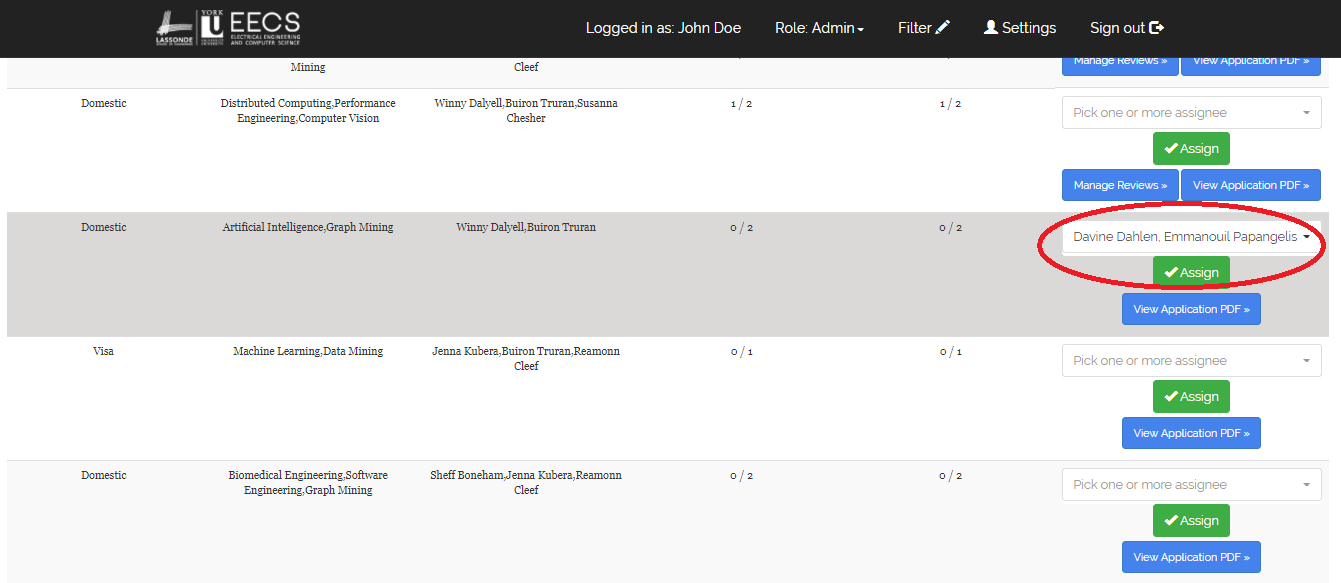
\includegraphics[width=.99\textwidth]{images/adm/mr/assign_review.png}
\end{center}
\caption{Assign a review}
\label{fig:adm/assign_review}
\end{figure}

\subsubsection{Unassign Review}
Once in the managing review portal, you can manage a review for the corresponding application. To manage the review, click on \emph{Manage Reviews} for the corresponding application. In the review outline page, it will display all the reviewers for the application. You can unassign a review for an application if it has not been submitted yet.

\begin{figure}[!htb]
\begin{center}
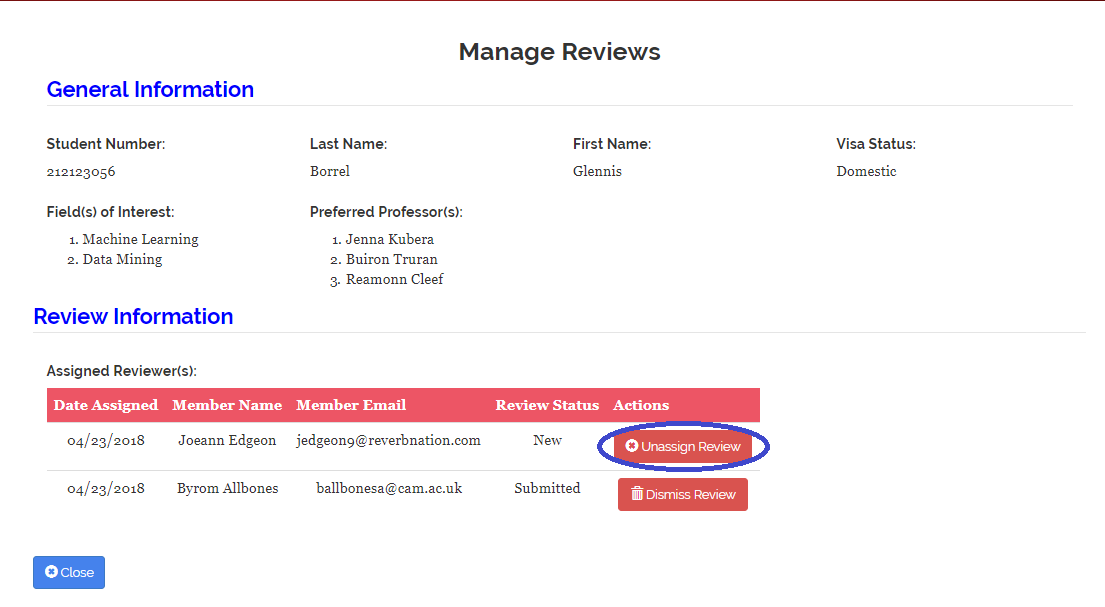
\includegraphics[width=.99\textwidth]{images/adm/mr/unassign_review.png}
\end{center}
\caption{Unassign a review}
\label{fig:adm/unassign_review}
\end{figure}

\clearpage
\subsubsection{Dismiss Review}
Once in the managing review portal, you can manage a review for the corresponding application. To manage the review, click on \emph{Manage Reviews} for the corresponding application. In the review outline page, it will display all the reviewers for the application. You can dismiss a review for an application if it has been already submitted.

\begin{figure}[!htb]
\begin{center}
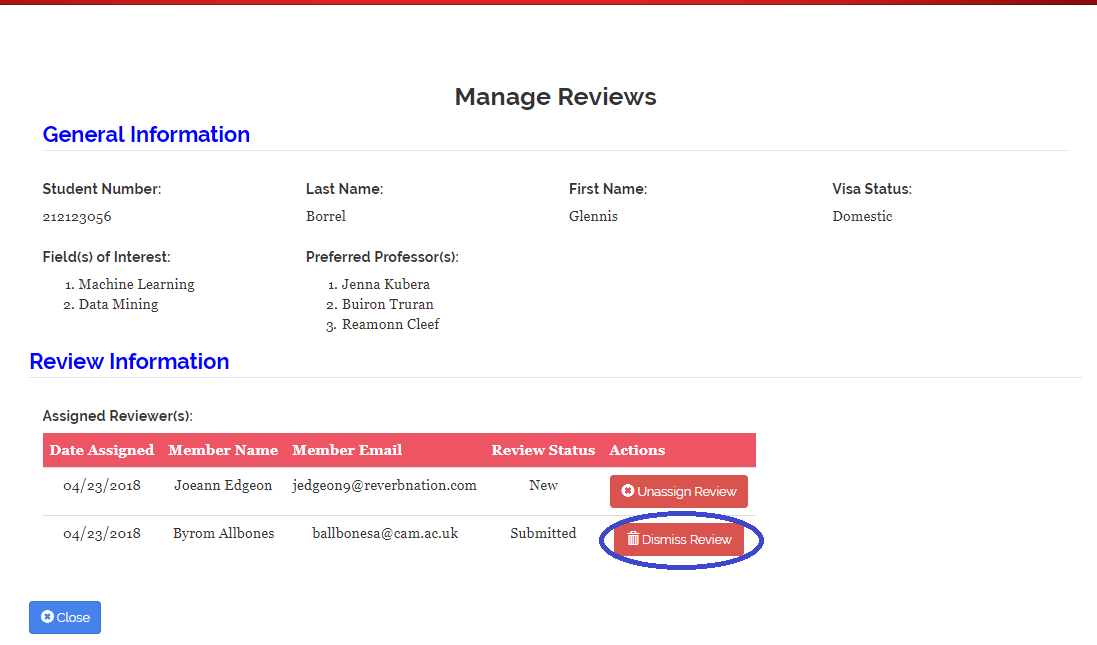
\includegraphics[width=.99\textwidth]{images/adm/mr/dismiss_review.png}
\end{center}
\caption{Dismiss a review}
\label{fig:adm/dismiss_review}
\end{figure}

\clearpage
\subsubsection{Filtering the Table}
This section describes how you would use/build a filter on the table.

\begin{enumerate}

\item \textbf{Opening the Modal} To begin with filtering you must open the modal. To do so click on the ``Filter" button on the navigation bar.

\begin{figure}[!htb]
\begin{center}
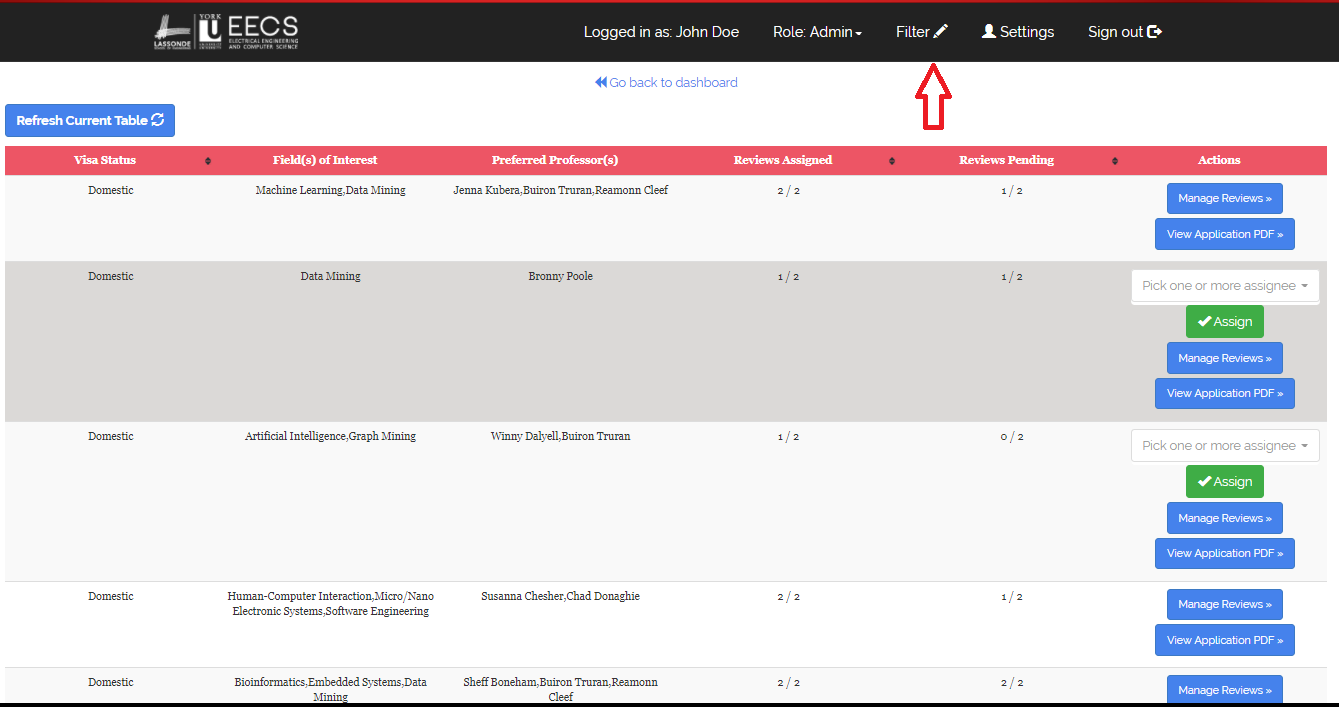
\includegraphics[width=.99\textwidth]{images/adm/mr/open_modal.png}
\end{center}
\caption{Opening the  Modal}
\label{fig:adm/open_modal}
\end{figure}

\clearpage
\newpage
\item \textbf{Choose Your Columns} Once the modal is opened you can then choose the columns you wish to be displayed on the table. To do so, click on the button indicating which column you wish to see. Once clicked the button will display the order that column will appear in the table.

\begin{figure}[!htb]
\begin{center}
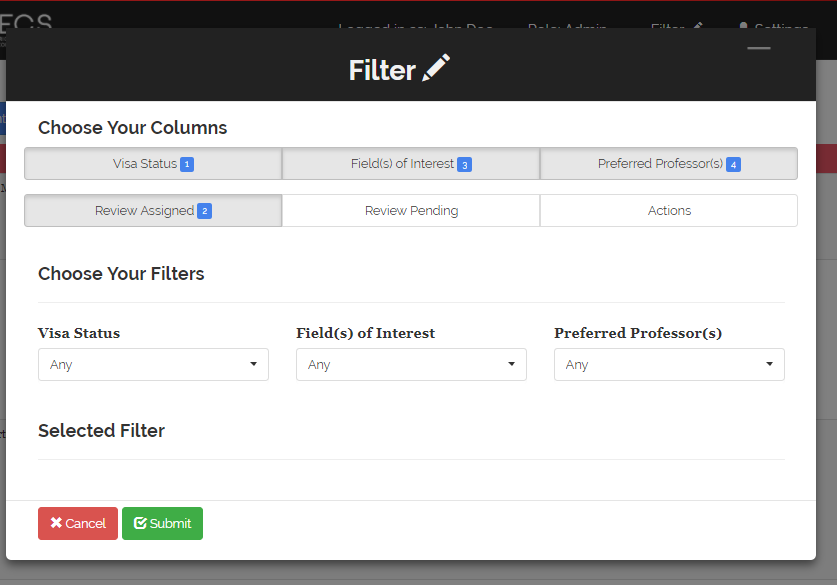
\includegraphics[width=.99\textwidth]{images/adm/mr/selected_col.png}
\end{center}
\caption{Choose Your Columns}
\label{fig:adm/choose_columns}
\end{figure}

\smallskip
\noindent \textbf{Note:} Not selecting any column will use the same columns and order as the default table. If the \emph{Actions} column is not selected it will automatically be placed as the right most column.

\clearpage
\item \textbf{Choose Your Filters} After selecting your columns, you can then choose the attributes by which you wish to filter your table. Begin by clicking on the drop down of the attribute you wish to filter and select an option from a list of generated options.

\begin{figure}[!htb]
\begin{center}
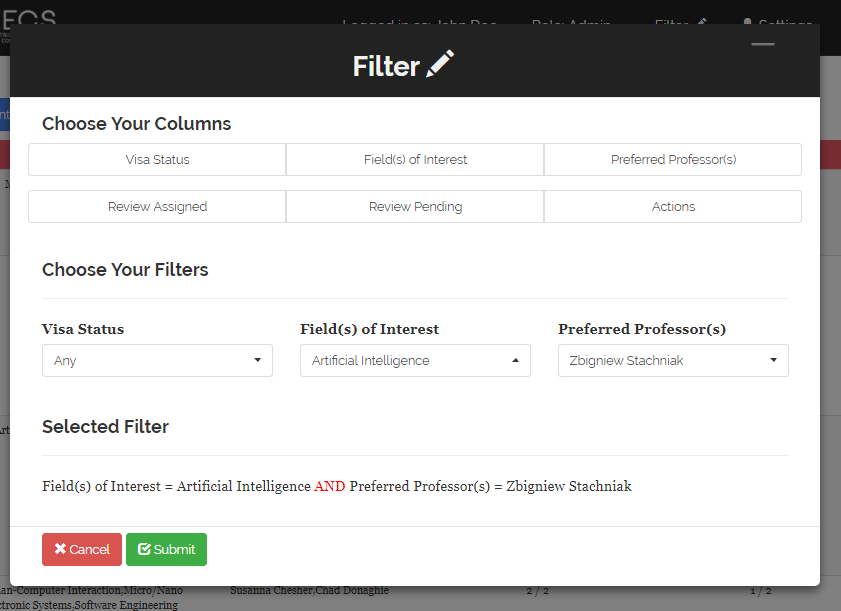
\includegraphics[width=.99\textwidth]{images/adm/mr/selected_filter.png}
\end{center}
\caption{Choose Your Filters}
\label{fig:adm/choose_filters}
\end{figure} 

\smallskip
\noindent \textbf{Note:} You can use the search bar to help locate values. Begin by typing in the text box displayed. You can only select an option that appears in the dropdown.

\clearpage
\item \textbf{Submitting a Filter} Once you have chosen your columns and filter attributes confirm your filter by reading the text under ``Selected Filter'' and click ``Submit". The text under the ``Selected Filter'' will change based on your filter attributes.

\bigskip
\noindent Once the resulting table is returned after filtering, you can assign/unassign/dismiss review from any of the returned applications.

\begin{figure}[!htb]
\begin{center}
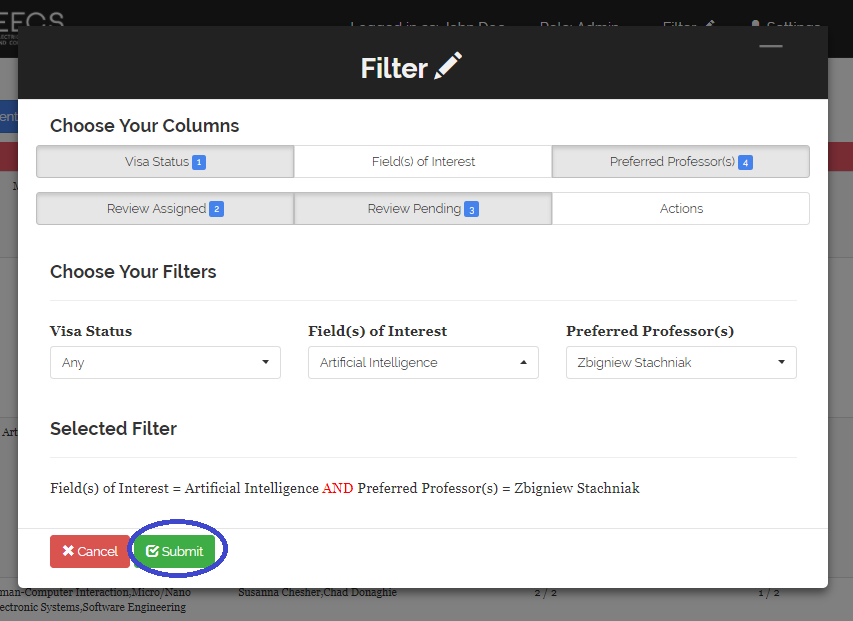
\includegraphics[width=.99\textwidth]{images/adm/mr/submit_filter.png}
\end{center}
\caption{Submit Filter}
\textbf{Note}: When submitting a filter with no selected filters, the default table will be loaded.
\label{fig:adm/submit_filter}
\end{figure}

\clearpage
\begin{figure}[!htb]
\begin{center}
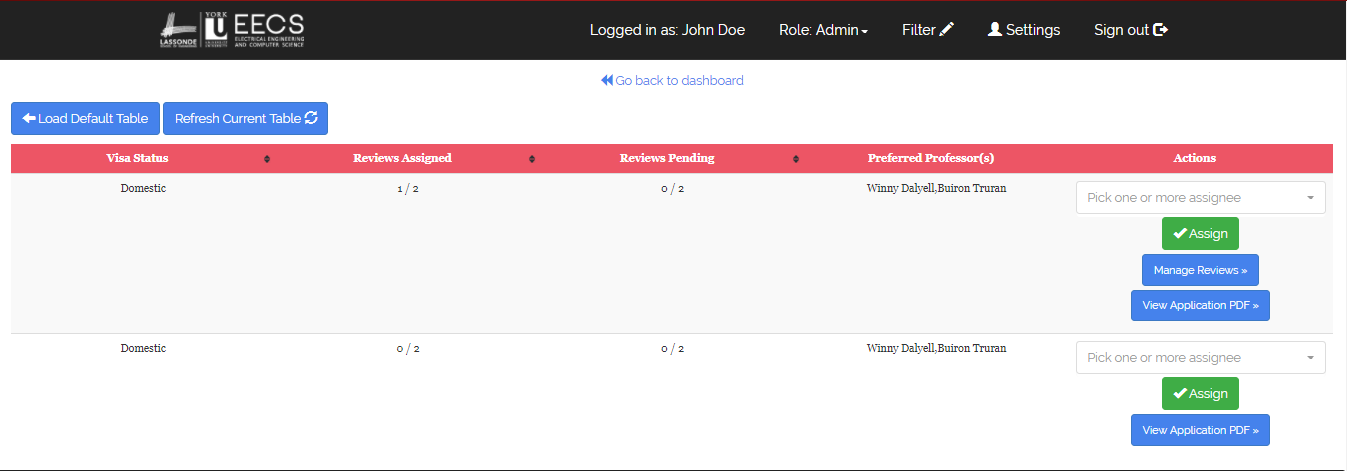
\includegraphics[width=.99\textwidth]{images/adm/mr/example_filter_table.png}
\end{center}
\caption{Resulted Table After Applying Filter}
\label{fig:adm/resulted_table}
\end{figure}

\end{enumerate}

\subsubsection{Sorting the Table}
If you wish to sort the table displayed simply click on the columns that display arrows next to the name. The table can be sorted in Ascending/Descending order described below.
\begin{itemize}
\item \textbf{Visa Status:} Descending Order = Z to A, Ascending order = A to Z
\item \textbf{Review Assigned:} Descending Order = Largest to Smallest, Ascending order = Smallest to Largest
\item \textbf{Review Pending:} Descending Order = Largest to Smallest, Ascending order = Smallest to Largest
\end{itemize}
\textbf{Pro-tip:} To sort by multiple columns hold the shift key while clicking on the columns.

\bigskip
\noindent \textbf{Note}: Ordering fields can be done on both filtered and unfiltered review application lists.

%%%%%%%%% COMMITTEE MEMBER MANUAL %%%%%%%%%%%
\clearpage
\newpage
\section{Committee Member}
This section provides a detailed description of the committee member system functions.

\subsection{Default Portal}
After logging in and selecting the \emph{Committee Member} role you will have access to the committee member portal. In this portal you will be presented with a table containing all the students who have applied to be a graduate student. Here you can perform the following:
\begin{itemize}
\item View current and past reviewed application(s)
\item Apply filters on current and past reviewed application(s)
\item Review an assigned application(s)
\item Save a review as a draft for later completion.
\item Add new university assessments in the system to be used in a review. Such a new assessment will be added globally to the system and can be seen and used by other committee members when filling out a review.
\end{itemize} 

\begin{figure}[!htb]
\begin{center}
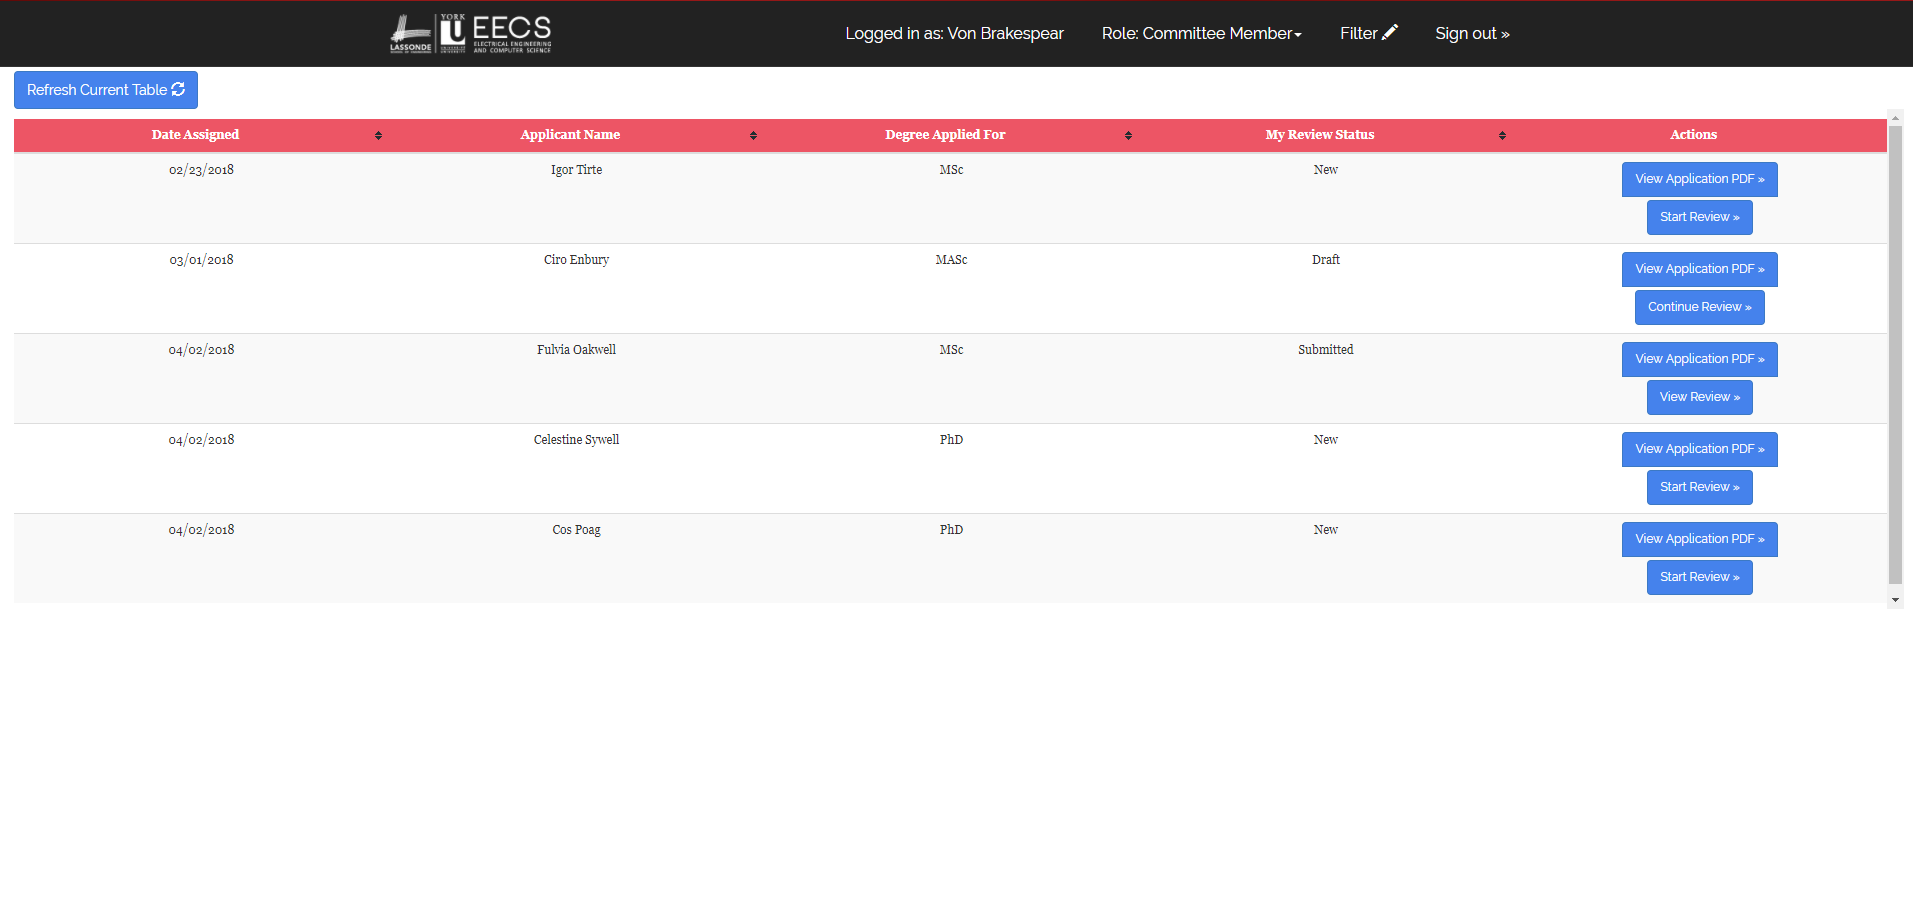
\includegraphics[width=.8\textwidth]{images/cm/default_table.png}
\end{center}
\caption{Committee Member Portal}
\label{fig:cm:cm_portal}
\textbf{Note:} If there are no reviews assigned, it will display a message instead. 
\end{figure}

\newpage
\subsection{Filtering the Table}
This section describes how you would use/build/save/load a filter on the table.
\begin{figure}[!htb]
\subsubsection{Opening the Modal}
To begin with filtering you must open the modal. To do so click on the ``Filter" button on the navigation bar.
\begin{center}
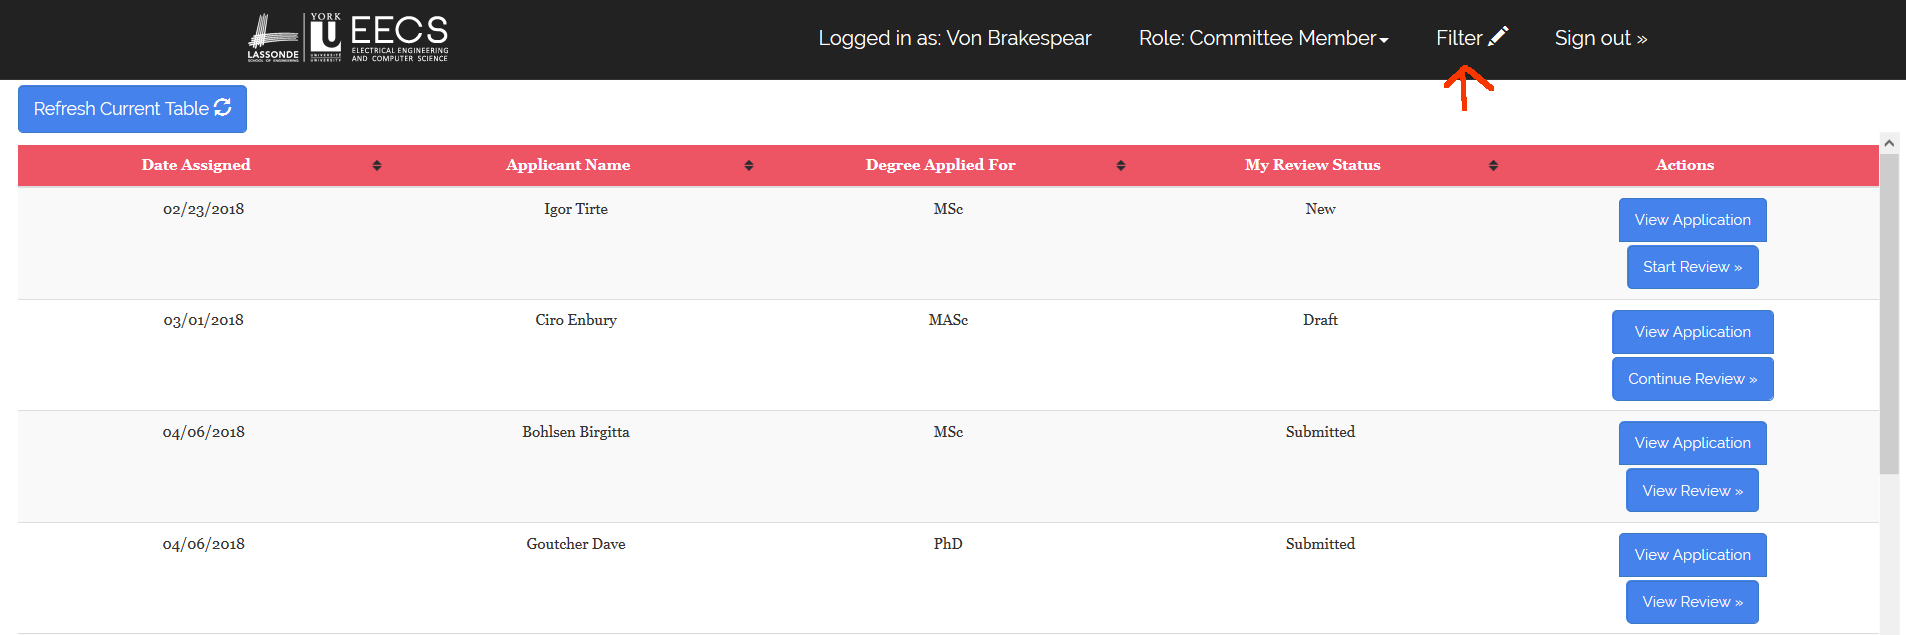
\includegraphics[width=.99\textwidth]{images/cm/open_modal.png}
\end{center}
\caption{Opening the  Modal}
\label{fig:cm:open_modal}
\end{figure}

\begin{figure}[!htb]
\begin{center}
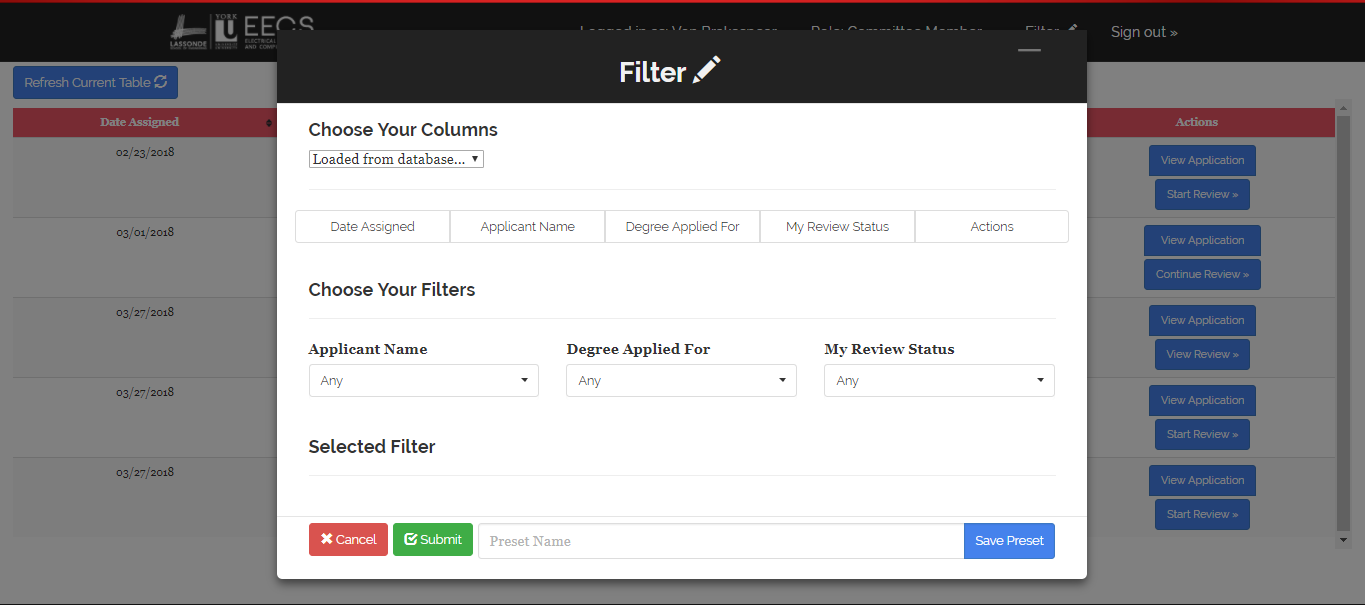
\includegraphics[width=.99\textwidth]{images/cm/default_filter_view.png}
\end{center}
\caption{Filter View}
\label{fig:cm:filter_view}
\end{figure}

\clearpage
\newpage

\begin{figure}[!htb]
\subsubsection{Choose Your Columns}
Once the modal is opened you can then choose the columns you wish to be displayed on the table. To do so, click on the button indicating which column you wish to see. Once clicked the button will display the order that column will appear in the table.\begin{center}
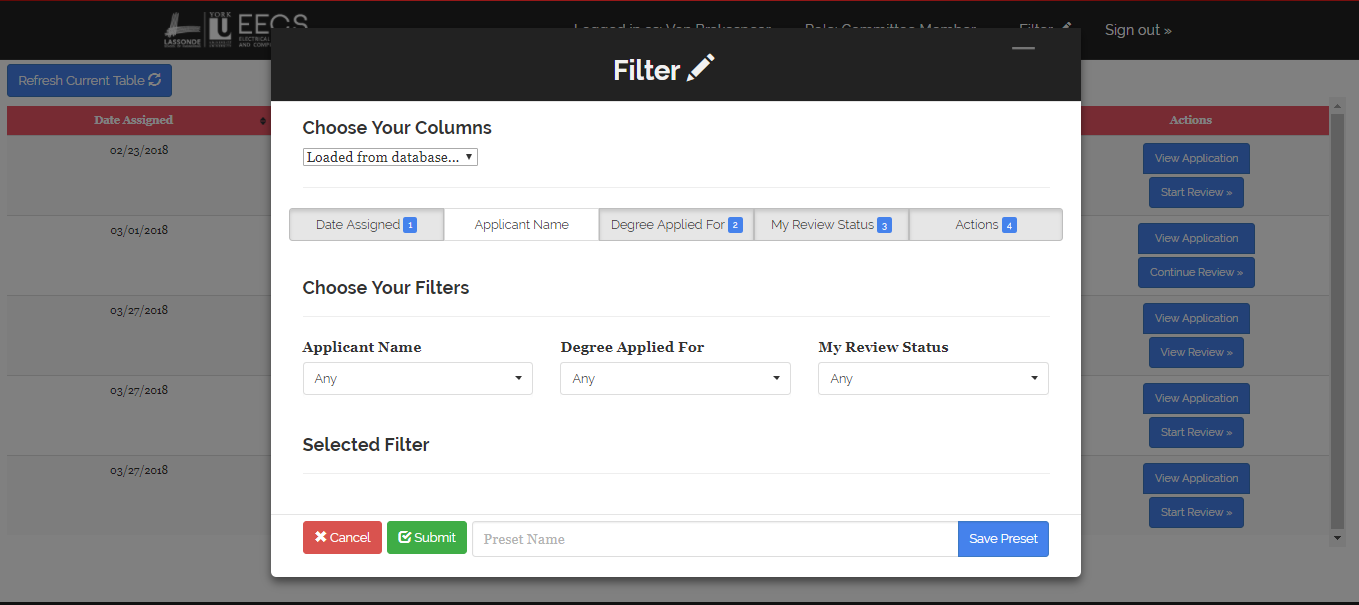
\includegraphics[width=.99\textwidth]{images/cm/selected_col.png}
\end{center}
\caption{Choose Your Columns}
\label{fig:cm:choose_columns}
\textbf{Note:} Not selecting any column will use the same columns and order as the default table. If the \emph{Actions} column is not selected it will automatically be placed as the right most column. 
\end{figure}

\clearpage
\begin{figure}[!htb]
\subsubsection{Choose Your Filters}
After selecting your columns, you can then choose the attributes by which you wish to filter your table. Begin by clicking on the drop down of the attribute you wish to filter and select an option from a list of generated options.
\begin{center}
\includegraphics[width=.99\textwidth]{images/cm/selected_filter.png}
\end{center}
\caption{Choose Your Filters}
\textbf{Note:} You can use the search bar to help locate values. Begin by typing in the text box displayed. You can only select an option that appears in the dropdown.
\label{fig:cm:choose_filters}
\end{figure} 

\clearpage 
\begin{figure}[!htb]
\subsubsection{Submitting a Filter}
Once you have chosen your columns and filter attributes confirm your filter by reading the text under ``Selected Filter'' and click ``Submit". The text under the ``Selected Filter'' will change based on your filter attributes.
\begin{center}
\includegraphics[width=.9\textwidth]{images/cm/submit_filter.png}
\end{center}
\caption{Submit Filter}
\textbf{Note}: When submitting a filter with no selected filters, the default table will be loaded.
\label{fig:cm:submit_filter}
\end{figure}

\begin{figure}[!htb]
\begin{center}
\includegraphics[width=.9\textwidth]{images/cm/example_filter_table.png}
\end{center}
\caption{Resulted Table After Applying Filter}
\label{fig:cm:resulted_table}
\end{figure}

\clearpage

\begin{figure}[!htb]
\subsubsection{Saving a Filter}
Once you have chosen your columns and filter attributes confirm your filter by reading the text under ``Selected Filter'' and give the preset a name by typing in the text box between the ``Submit'' and the ``Save Preset'' button. Once that is done click ``Save Preset''.
\begin{center}
\includegraphics[width=.99\textwidth]{images/cm/saving_preset.png}
\end{center}
\caption{Save a Filter}
Once you have saved a filter you will be provided with a new table to match your filter and it will appear in the dropdown to be used for loading a filter.\\
\textbf{Pro-tip:} You can update a filter by typing in the same name as an existing filter.
\label{fig:cm:save_filter}
\end{figure}
\clearpage
\subsubsection{Deleting a Filter}
You can delete a filter by going into your settings. See Section \ref{user-settings}.
\begin{figure}[!htb]
\subsubsection{Loading a Filter}
To load a saved filter click the dropdown under ``Load a Preset'' and select the preset you wish to use. Once selected the modal will auto-populate.
\begin{center}
\includegraphics[width=.99\textwidth]{images/cm/load_preset.png}
\end{center}
\caption{Loading a Filter}
\textbf{Pro-tip:} Create a preset called \emph{Default} with no columns or filters selected. You can then use this to load the default table or help clear any data you put in the modal.
\label{fig:cm:save_filter}
\end{figure}
\clearpage
\newpage
\subsection{Sorting the Table}
If you wish to sort the table displayed simply click on the columns that display arrows next to the name. The table can be sorted in Ascending/Descending order described below.
\begin{itemize}
\item \textbf{Name:} Descending Order = Z to A, Ascending order = A to Z
\item \textbf{Date Assigned:} Descending Order = Newest - Oldest, Ascending order = Oldest - Newest
\item \textbf{Degree Applied For:} Descending Order = Z to A, Ascending order = A to Z
\item \textbf{Review Status:} Descending Order = Z to A, Ascending order = A to Z
\end{itemize}
\textbf{Pro-tip:} To sort by multiple columns hold the shift key while clicking on the columns.


\bigskip
\noindent \textbf{Note}: Ordering fields can be done on both filtered and unfiltered review application lists.

\bigskip
\noindent The following images depict how to order review applications using the \emph{Date Assigned} field in ascending and descending order.

\begin{figure}[!htb]
\begin{center}
\includegraphics[width=.99\textwidth]{images/cm/order_ascending.png}
\end{center}
\caption{Ascending order of Date Assigned field}
\label{fig:cm:order_ascending}
\end{figure}

\begin{figure}[!htb]
\begin{center}
\includegraphics[width=.99\textwidth]{images/cm/order_descending.png}
\end{center}
\caption{Descending order of Date Assigned field}
\label{fig:cm:order_descending}
\end{figure}

\newpage

\begin{figure}[!htb]
\begin{center}
\includegraphics[width=.99\textwidth]{images/cm/multiple_order.png}
\end{center}
\caption{Ordering using multiple fields}
\label{fig:cm:multiple_order}
\end{figure}

\clearpage
\newpage
\subsection{Reviewing Applications} \label{sec:reviews}
The review process can have \textbf{three} different statuses shown
\begin{itemize}
\item \textbf{New}: A new application has been assigned to the committee member and no changes have been made on the review yet.
\item \textbf{Draft}: A previously saved draft review. A review is considered as a draft when there has been at least one or more changes committed and the user has decided to save the changes.
\item \textbf{Submitted}: A completed review which has been submitted and uploaded to the server. Once a review is submitted, it cannot be undone.
\end{itemize}

\bigskip
\noindent The following list denotes the fields in a review form that is \textbf{not} submitted yet and their requirement status:
\begin{table}[h]
\centering
\begin{tabular}{|c | c |}
	\cline{1-2}
	\textbf{Field Name} & \textbf{Required}\\ \hline
	Institution Name(s) & No \\ \hline
	Institution Assessment(s) & No \\ \hline
	Background Information & No \\ \hline
	Research Experience & No \\ \hline
	Letter of Intent Analysis & No \\ \hline
	Additional Comments & No \\ \hline
	Applicant Rank & Yes \\ \hline
\end{tabular}
\caption {Review Fields}
\label{tbl:cm:review_fields}
\end{table}

\newpage
\bigskip
\noindent The following image depicts the full view of the review form. The \emph{View Application PDF} link opens the student application in PDF version uploaded by the system administrator. 

\begin{figure}[!htb]
\begin{center}
\includegraphics[width=.99\textwidth]{images/cm/review_form.png}
\end{center}
\caption{Full view of the Review Form}
\label{fig:cm:review_form}
\end{figure}

\clearpage
\newpage
\subsubsection{Opening a new Review}
When a new review is received it will show on the portal. After that you will have the option of opening the review and start completing the form. The action for opening a new review will say \textbf{Start Review}.

\bigskip
\noindent The following image depicts user opening a brand new review.

\begin{figure}[!htb]
\begin{center}
\includegraphics[width=.99\textwidth]{images/cm/opening_new_review.png}
\end{center}
\caption{Opening a brand new review}
\label{fig:cm:opening_new_review}
\end{figure}

\bigskip
\noindent The following image depicts user making no changes to the opened review and exiting out of the review form.

\begin{figure}[!htb]
\begin{center}
\includegraphics[width=.99\textwidth]{images/cm/new_review_exit_wo_changes.png}
\end{center}
\caption{Exiting out of a brand new review application without changes}
\label{fig:cm:new_review_exit_w/o_changes}
\end{figure}

\subsubsection{Filling out a Review}
Table \ref{tbl:cm:review_fields} outlines the fields in a review application and their required status. The following table specializes Table \ref{tbl:cm:review_fields} and displays the type of input each field takes.

\begin{table}[h]
\centering
\begin{tabular}{|c | c |}
	\cline{1-2}
	\textbf{Field Name} & \textbf{Input Type}\\ \hline
	Institution Name(s) & Multiple Drop-Down \\ \hline
	Institution Assessment(s) & Multiple Drop-Down \\ \hline
	Background Information & Text \\ \hline
	Research Experience & Text \\ \hline
	Letter of Intent Analysis & Text \\ \hline
	Additional Comments & Text \\ \hline
	Applicant Rank & Single Drop-Down \\ \hline
\end{tabular}
\caption {Review Fields Input Type}
\label{tbl:cm:review_fields_input}
\end{table}

\bigskip
\noindent \textbf{Institution Assessment}: When performing an institution assessment you can select from one or more institutions and a description in the database. If the institution does not exist or their description is inadequate you can also create a new institution/assessment.

\bigskip
\noindent The following image depicts a user selecting two institutions the applicant has attended and selecting an assessment from each of the institutions.

\begin{figure}[!htb]
\begin{center}
\includegraphics[width=.7\textwidth]{images/cm/uni_assessment.png}
\end{center}
\caption{Institution Assessment View}
\label{fig:cm:uni_assessment}
\end{figure}

\clearpage
\newpage
\subsubsection{Saving a Review as Draft}
While filling out a review you will have the opportunity to save an on-going review as a draft for future completion.

\bigskip
\noindent The following images depicts a user making changes to an application review and then saving it as a draft. Consequently, the status of the review is changed to \textbf{Draft}. And if the user wants to continue working on the draft sometime later, the action for opening a drafted review will say \textbf{Continue Review}.

\begin{figure}[!htb]
\begin{center}
\includegraphics[width=.9\textwidth]{images/cm/save_as_draft_review.png}
\end{center}
\caption{Save a review as draft}
\label{fig:cm:save_as_draft_review}
\end{figure}

\begin{figure}[!htb]
\begin{center}
\includegraphics[width=.9\textwidth]{images/cm/drafted_review.png}
\end{center}
\caption{Drafted Review View}
\label{fig:cm:drafted_review}
\end{figure}

\clearpage
\subsubsection{Submitting a Review}
Once you are satisfied with your review simply  click the \textbf{Submit Review} button to complete your review. If the correct number of reviews for an application has been submitted (depending on visa status), the application will be automatically available for selection to those on the \textbf{Professor Portal}. The only required field needed for submitting a review is the final application rank that is to be decided by the admission committee member upon analysing the application.

\bigskip
\noindent The following image depicts an end user submitting a review. 

\begin{figure}[!htb]
\begin{center}
\includegraphics[width=.8\textwidth]{images/cm/submit_review.png}
\end{center}
\caption{Submit a Review}
\label{fig:cm:submit_review}
\end{figure}
\clearpage
\bigskip
\noindent Once the review is submitted, it will show up on the user dashboard with status as \textbf{Submitted} and the user action to view a submitted review will say \textbf{View Review}. Submitted reviews are only viewable as a plain text application form. The following images depict viewing a submitted review.

\begin{figure}[!htb]
\begin{center}
\includegraphics[width=.8\textwidth]{images/cm/submitted_review.png}
\end{center}
\caption{Submitted Review View}
\label{fig:cm:submitted_review}
\end{figure}

\begin{figure}[!htb]
\begin{center}
\includegraphics[width=.8\textwidth]{images/cm/submit_review_view.png}
\end{center}
\caption{Submitted Review View}
\label{fig:cm:submit_review_view}
\end{figure}

%%%%%%%%%% PROFESSOR MANUAL %%%%
\clearpage
\newpage
\section{Professor}
This section provides a detailed description of the professor system functions.

\subsection{Default Portal}
After logging in and selecting the professor role you will have access to the professor portal. In this portal you will be presented with a table containing all the students who have applied to be a graduate student. Here you can perform the following:
\begin{itemize}
\item Filter the table to only display applications based on criteria of your choosing
\item Sort the table on certain columns
\item View applications and their respective committee review
\item Set application attributes such as notifying others if you have contacted/requested an applicant or indicate to yourself if you find an applicant interesting or not.
\end{itemize}

\subsection{Filtering the Table}
This section describes how you would use/build/save/load a filter on the table.

\newpage
\subsubsection{Opening the Modal}
To begin with filtering you must open the modal. To do so click on the ``Filter" button on the navigation bar.

\begin{figure}[!htb]
\begin{center}
\includegraphics[width=.99\textwidth]{images/prof/open_modal.png}
\end{center}
\caption{Opening the  Modal}
\label{fig:prof/open_modal}
\end{figure}

\clearpage
\begin{figure}[!htb]
\begin{center}
\includegraphics[width=.99\textwidth]{images/prof/filter_view.png}
\end{center}
\caption{Filter View}
\label{fig:prof/filter_view}
\end{figure}

\clearpage
\begin{figure}[!htb]
\subsubsection{Choose Your Columns}
Once the modal is opened you can then choose the columns you wish to be displayed on the table. To do so, click on the button indicating which column you wish to see. Once clicked the button will display the order that column will appear in the table.\begin{center}
\includegraphics[width=.99\textwidth]{images/prof/choose_columns.png}
\end{center}
\caption{Choose Your Columns}
\label{fig:prof/choose_columns}
\textbf{Note:} Not selecting any column will use the same columns and order as the default table. If the \emph{Actions} column is not selected it will automatically be placed as the right most column. \emph{My Interest Status} is account specific and can only be seen by you.
\end{figure}

\clearpage

\begin{figure}[!htb]
\subsubsection{Choose Your Filters}
After selecting your columns, you can then choose the attributes by which you wish to filter your table. Begin by clicking on the drop down of the attribute you wish to filter and select an option from a list of generated options.
\begin{center}
\includegraphics[width=.99\textwidth]{images/prof/choose_filters.png}
\end{center}
\caption{Choose Your Filters}
\textbf{Note:} You can use the search bar to help locate values. Begin by typing in the text box displayed. You can only select an option that appears in the dropdown.
\label{fig:prof/choose_filters}
\end{figure}

\clearpage 
\begin{figure}[!htb]
\subsubsection{Submitting a Filter}
Once you have chosen your columns and filter attributes confirm your filter by reading the text under ``Selected Filter'' and click ``Submit". The text under the ``Selected Filter'' will change based on your filter attributes.
\begin{center}
\includegraphics[width=.99\textwidth]{images/prof/submit_filter.png}
\end{center}
\caption{Submit Filter}
\label{fig:prof/submit_filter}
\end{figure}

\clearpage
After you submit a filter you will be provided with a new table to match your filter.
\begin{figure}[!htb]
\begin{center}
\includegraphics[width=.99\textwidth]{images/prof/filtered_table.png}
\end{center}
\caption{Filtered Table}
\textbf{Pro-tip:} Attributes that satisfy your filter will be highlighted. Make sure to include the right column to see those highlights!
\label{fig:prof/filtered_table}
\end{figure}

\clearpage 

\begin{figure}[!htb]
\subsubsection{Saving a Filter}
Once you have chosen your columns and filter attributes confirm your filter by reading the text under ``Selected Filter'' and give the preset a name by typing in the text box between the ``Submit'' and the ``Save Preset'' button. Once that is done click ``Save Preset''.
\begin{center}
\includegraphics[width=.99\textwidth]{images/prof/save_filter.png}
\end{center}
\caption{Save a Filter}
Once you have saved a filter you will be provided with a new table to match your filter and it will appear in the dropdown to be used for loading a filter.\\
\textbf{Pro-tip:} You can update a filter by typing in the same name as an existing filter.
\label{fig:prof/save_filter}
\end{figure}

\clearpage
\subsubsection{Deleting a Filter}
You can delete a filter by going into your settings. See Section \ref{user-settings}.
\begin{figure}[!htb]
\subsubsection{Loading a Filter}
To load a saved filter click the dropdown under ``Load a Preset'' and select the preset you wish to use. Once selected the modal will auto-populate.
\begin{center}
\includegraphics[width=.99\textwidth]{images/prof/load_filter.png}
\end{center}
\caption{Loading a Filter}
\textbf{Pro-tip:} Create a preset called \emph{Default} with no columns or filters selected. You can then use this to load the default table or help clear any data you put in the modal.
\label{fig:prof/save_filter}
\end{figure}

\clearpage

\subsection{Sorting the Table}
If you wish to sort the table displayed simply click on the columns that display arrows next to the name. The table can be sorted in Ascending/Descending order described below.
\begin{itemize}
\item \textbf{Name:} Descending Order = Z to A, Ascending order = A to Z
\item \textbf{Gender:} Descending Order = Z to A, Ascending order = A to Z
\item \textbf{Committee Rank:} Descending Order = A+ to C, Ascending order = C to A+
\item \textbf{GPA:} Descending Order = A+ to C, Ascending order = C to A+
\item \textbf{Degree Applied For:} Descending Order = Z to A, Ascending order = A to Z
\item \textbf{Visa Status:} Descending Order = Z to A, Ascending order = A to Z
\item \textbf{Program Decision:} Descending Order = Z to A, Ascending order = A to Z
\item \textbf{Interest Status:} Descending Order = Z to A, Ascending order = A to Z
\end{itemize}
\textbf{Pro-tip:} To sort by multiple columns hold the shift key while clicking on the columns. For example to sort by Committee Rank and then GPA, hold onto shift and left click Committee Rank and then GPA.
\begin{figure}[!htb]
\begin{center}
\includegraphics[width=.99\textwidth]{images/prof/sorted_table.png}
\end{center}
\caption{Sort Table}
\label{fig:prof/sorted_table}
\end{figure}
\clearpage
\subsection{Viewing an Application}
To view an application click on ``View Application'' at the row corresponding to the applicant you wish to view.
\begin{figure}[!htb]
\begin{center}
\includegraphics[width=.99\textwidth]{images/prof/view_app.png}
\end{center}
\caption{Viewing an Application}
\end{figure}
\begin{figure}[!htb]
You will be redirected to an application summary page that will contain a summary of the application and the committee review. If you wish to see more click on ``View Application PDF".
\begin{center}
\includegraphics[width=.99\textwidth]{images/prof/viewapp.png}
\end{center}
\caption{Application Summary}
\label{fig:prof/sorted_table}
\end{figure}
\clearpage

\subsection{Setting Application Attributes}
Clicking on the ``Set To" drop down on an applicant row will provide you options to update the following fields on an application.
\begin{itemize}
\item \textbf{Contacted/Requested:} Indicate to others whether or not you have contacted/requested a student (default not contacted and not requested).
\item \textbf{My Interest Status:} This is a personal field to help you keep track of applications you have/haven't viewed and your opinion of them. It can only be seen by you.
\end{itemize}

\begin{figure}[!htb]
\begin{center}
\includegraphics[width=.99\textwidth]{images/prof/set_attribute.png}
\end{center}
\caption{Setting Application Attribute}
\label{fig:prof/set_attribute}
\end{figure}

\begin{figure}[!htb]
\begin{center}
\includegraphics[width=.99\textwidth]{images/prof/set_attribute2.png}
\end{center}`
\caption{Results}
\label{fig:prof/set_attribute_results}
\end{figure}

\clearpage
\newpage
\section{Help}
For further help or information about GradApps 2.0 please contact the Graduate Program Director (GPD) or the Graduate Program Assistant (GPA) of the EECS Graduate Program at Lassonde School of Engineering.\\

\begin{center}
\begin{tabular}{ |c |c |c | } \hline
 \textbf{Role} & \textbf{Name} & \textbf{Contact} \\ \hline
 Graduate Program Director & Franck van Breugel & gpd@eecs.yorku.ca \\ \hline
 Graduate Program Assistant & Ouma Jaipaul-Gill & gpa@eecs.yorku.ca \\ \hline
\end{tabular}
\end{center}

\end{document}
